% Define document class
\documentclass[twocolumn]{aastex631}
\usepackage{showyourwork}

\newcommand{\sbu}{Department of Physics and Astronomy, Stony Brook University, Stony Brook NY 11794, USA}
\newcommand{\cca}{Center for Computational Astrophysics, Flatiron Institute, New York NY 10010, USA}
\renewcommand{\thefigure}{\arabic{figure}}

\usepackage{bbold}

% Begin!
\begin{document}

% Title
\title{Polka-dotted Stars: a Hierarchical Model for Mapping Stellar Surfaces Using Occultation Light Curves and the Case of TOI-3884}

% Author list
\author[0000-0002-6650-3829]{Sabina Sagynbayeva}
\email{sabina.sagynbayeva@stonybrook.edu}
\affiliation{\sbu}
\affiliation{\cca}

\author[0000-0003-1540-8562]{Will M. Farr}
% \email{wfarr@flatironinstitute.org}
\affiliation{\sbu}
\affiliation{\cca}

\author[0000-0002-0296-3826]{Rodrigo Luger}
% \email{rodluger@gmail.com}
\affiliation{\cca}

% Abstract with filler text
\begin{abstract}
   
\end{abstract}

% Main body with filler text
\section{Introduction}
\label{sec:intro}
The quest to unravel the mysteries of distant planetary systems has led to a fast-evolving field of research, where exoplanet studies are at the forefront of 
astronomical investigations. The detection of atmospheres on Earth analogs using transmission spectroscopy is a challenging task due to the confounding 
effects of stellar contamination (see, e.g., \cite{Ducrot2018, Morris2018}). Stellar magnetic activity, particularly in the form of starspots, can significantly 
influence the observed transmission spectra, making it difficult to disentangle planetary atmospheric signals from those originating from the host star. 
Starspots exhibit variations in both time and wavelength, mainly due to stellar rotation. As a result, the identification of starspots has the potential to 
complicate the analysis and interpretation of exoplanet observations. 

Therefore, characterizing the behavior of stellar surface features that arise due to magnetic activity like starspots and flares is instrumental for improving 
planet detection efficiency in photometric, spectral, and radial velocity studies. Understanding starspots is fundamental and imminent for the ongoing 
space mission JWST, which will characterize tens to hundreds of exoplanet atmospheres around stars with strong variability. In fact, recent JWST 
results (\cite{Lim2023}) on the atmosphere of TRAPPIST-1b showed that accurate measurements have so far been substantially stymied by stellar contamination, 
and we need more accurate models to account for it. To fully capitalize on the unprecedented capabilities of JWST and accurately interpret the obtained 
transmission spectra, it is crucial to develop a comprehensive understanding of stellar magnetic activity and its impact on the observed signals. 

Moreover, characterizing the surfaces of exoplanet-host stars is crucial for understanding the environments and evolution of their planetary 
systems. For example, the Sun's magnetic field drives the star's activity cycles, the heating of its outer atmosphere and the solar wind,
which affects the Earth's magnetosphere and biosphere \citep{Babcock1961,Charbonneau2014}. 
Therefore, constructing a catalogue of the magnetic properties of other stars similar to the Sun would support the quest towards understanding 
the population of detected exoplanets and the development of a highly generalizable theory on stellar magnetic dynamo.

The reverse statement is also true. The exisiting popultion of exoplanets along with their orbital parameters can help characterize their host-stars
in terms of their surface magnetic activity. Stellar surface features like spots and flares impact observables in planet-detection research including photometric 
variability, spectral line profiles, and radial velocity shifts. However, directly resolving stellar surfaces remains challenging. 
While high-resolution spectroscopy provides the most robust method of determining stellar parameters, obtaining such data for large samples remains 
observationally expensive, but photometric observations can come to rescue. Some recent works offered invaluable insights into the topographical 
characteristics of stars and their magnetic activity, responsible for the observed variatians on their surfaces. For example, the influence of starspots 
can be seen through photometric data acquired from Kepler or TESS. \cite{Luger2021b} investigated the star spots features on the stellar surfaces using 
Gaussian Process (GPs) with a \emph{physically interpretable} kernel. They argue that the complex degeneracies make it impossible to determine the 
precise configuration of starspots and other features on a star's surface solely based on its rotational light curve, but we don't have to be 
concerned with the specific characteristics of an individual spot, as such information would have limited practical utility. Instead, we often consider 
(either explicitly or implicitly) the properties of a star spot as a sample drawn from an underlying parent distribution that governs aspects like the average 
and dispersion of spot radii. The parameters that control this distribution are the ones that can be predicted through physical principles, 
making them the primary focus of our interest. 

\cite{Luger2021b} also showed that it is hard to put constrains on starspot properties if you only have a light curve for 
one star, it is rather usefule though to perform the same analysis for an ensemble of stars. However, photometric light curves capturing planetary transits encode 
a wealth of information about the stellar surface and the starspots present on it. Transits, during which the planet occults different regions of 
the stellar disk, provide a unique opportunity to probe the physical characteristics of starspots. Exoplanet host stars are \textit{uniquely} suited 
for photometric studies of starspot properties: spot features of observed exoplanet host stars in transit can provide valuable 
constraints on spot properties (see Figure \ref{fig:cartoon}) -- brightness, size, and latitude -- while fitting a single light curve for a star 
with no observed transit introduces too many degeneracies.

In this work, we utilize two powerful computational tools, \texttt{starry} and \texttt{StarryProcess}, to model the light curves of spotted stars and 
their transiting exoplanets. We then extend these models to create a comprehensive framework that combines both stellar variability and planetary transits.

The \texttt{starry} code, developed by \cite{Luger2019}, provides an efficient method for computing light curves of stars and planets. 
It uses a spherical harmonic framework to represent the surface brightness distribution of celestial bodies, allowing for fast and accurate 
calculations of rotational light curves and occultations. \texttt{starry} is particularly useful for modeling the effects of stellar spots 
and planetary transits, as it can handle complex surface brightness patterns and compute their resulting light curves with high precision.

Building upon \texttt{starry}, \cite{Luger2021b} introduced \texttt{StarryProcess}, a probabilistic model for stellar variability. \texttt{StarryProcess} 
treats the distribution of spots on a stellar surface as a Gaussian process in spherical harmonic space. This approach allows for the efficient 
modeling of stellar variability over long time scales, accounting for the evolution and rotational modulation of starspots. \texttt{StarryProcess} 
provides a flexible framework for inferring stellar and starspot properties.

Our model combines the capabilities of both \texttt{starry} and \texttt{StarryProcess}, integrating them with a transit model to 
create a comprehensive framework for analyzing light curves of spotted stars with transiting exoplanets. By leveraging the spherical harmonic 
representation from \texttt{starry} and the probabilistic approach of \texttt{StarryProcess}, we can simultaneously model the stellar variability, 
spot distribution, and planetary transits. This combined approach allows us to account for the effects of stellar spots on transit light curves, 
including spot-crossing events, while also constraining the overall stellar variability pattern. This integrated model enables us to derive more 
accurate and precise constraints on both stellar and planetary parameters. It accounts for the interplay between stellar activity and planetary transits, 
allowing us to disentangle the effects of spots from true transit features. Furthermore, by modeling multiple transits simultaneously with the 
underlying stellar variability, we can better constrain parameters such as stellar inclination, obliquity, and spot distribution, 
while also improving our estimates of planetary properties.

\begin{figure*}[hbt!]
    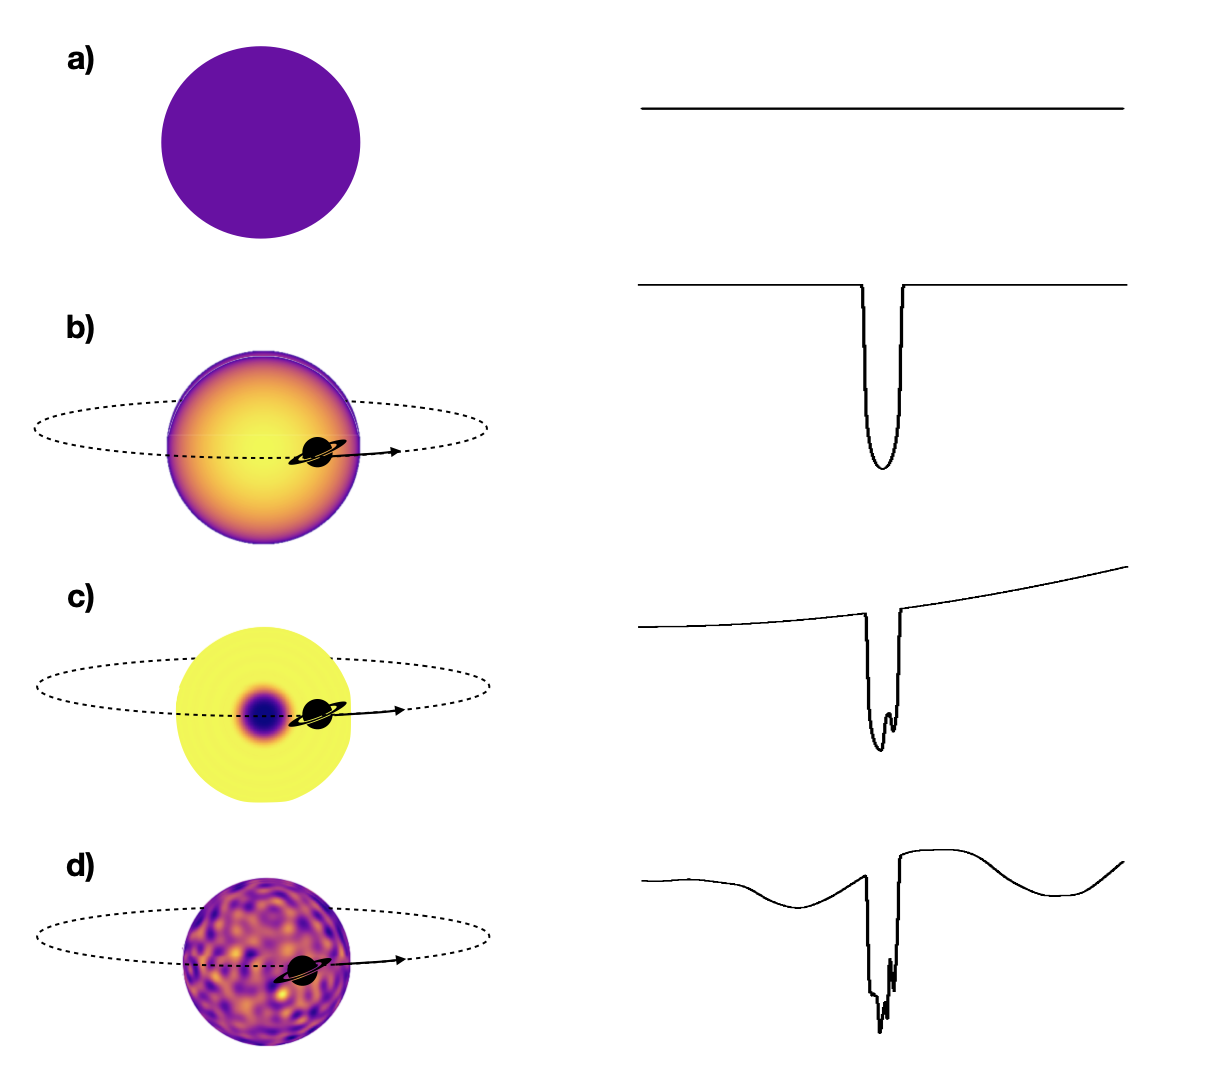
\includegraphics[width=\textwidth]{figures/star-planet-cartoon.png}
        \caption{Light curves from the kinds of stars shown on the left panel (these light curves were calculated analytically 
        using \texttt{starry} \citep{Luger2019}): (a) the light curve shows a flat flux if the star has no surface features and no planet orbiting it; 
        (b) a transit in the light curve of the star that hosts an exoplanet; (c) if the star has one orbiting planet and one starspot under the planet's 
        trajectory then it is seen as a bump in a transit signal; (d) the light curve becomes complicated when the star has multiple spots.}
        \label{fig:cartoon}
    \end{figure*}

The light curves obtained from telescopic observations often provide insufficient information for comprehensive photometric studies of stellar 
magnetic fields, yet they also yield an overabundance of data for simple forward modeling. To address the first issue, we focus on capturing the essence 
of the variability caused by the magnetic dynamo rather than solving it in great detail (as per the argument in \cite{Luger2021b}). The second challenge can 
be overcome by marginalizing over (integrating out) the properties of each individual spot on a star to infer the characteristics of the overall spot distribution. 
This could be accomplished by modeling the properties of each spot and generating 
the corresponding light curves with a model like \texttt{starry}, which does exactly that by constructing a disk-integrating signal 
with spherical harmonics. Then one can use a posterior sampling scheme, such as Markov Chain Monte Carlo (MCMC), 
while incorporating hyperparameters that control the distribution of spot properties across the entire population. The marginal posteriors for 
the hyperparameters would ultimately provide the information we seek. Bayesian modeling provides a principled framework for incorporating prior 
knowledge and uncertainties into the inference process, allowing us to robustly estimate the hyperparameters governing the distribution of star spot 
properties while naturally accounting for the complex degeneracies and multi-modality inherent in the problem.
However, in practice, the degeneracies and often extreme multi-modality of the distributions of individual spot properties would render this approach 
quite challenging and computationally expensive. That's why we harness the elegant machinery like Gaussian processes (GPs) to perform 
this marginalization on our behalf, simplifying the process and reducing the computational burden.

In Figure \ref{fig:nullspace}, we present an analysis similar to Figure 4 in \cite{Luger2021b}, but with the addition of a planetary transit. 
This figure illustrates the decomposition of a stellar surface map with a transiting planet into its preimage and null space components, 
along with their corresponding contributions to the light curve. Crucially, we observe that the planetary trajectory covers the visible part in the preimage 
component but absent in the null space. The transit path effectively "carves out" a strip on the stellar surface in nullspace but that is 
fully contained within the preimage.

\begin{figure*}[hbt!]
    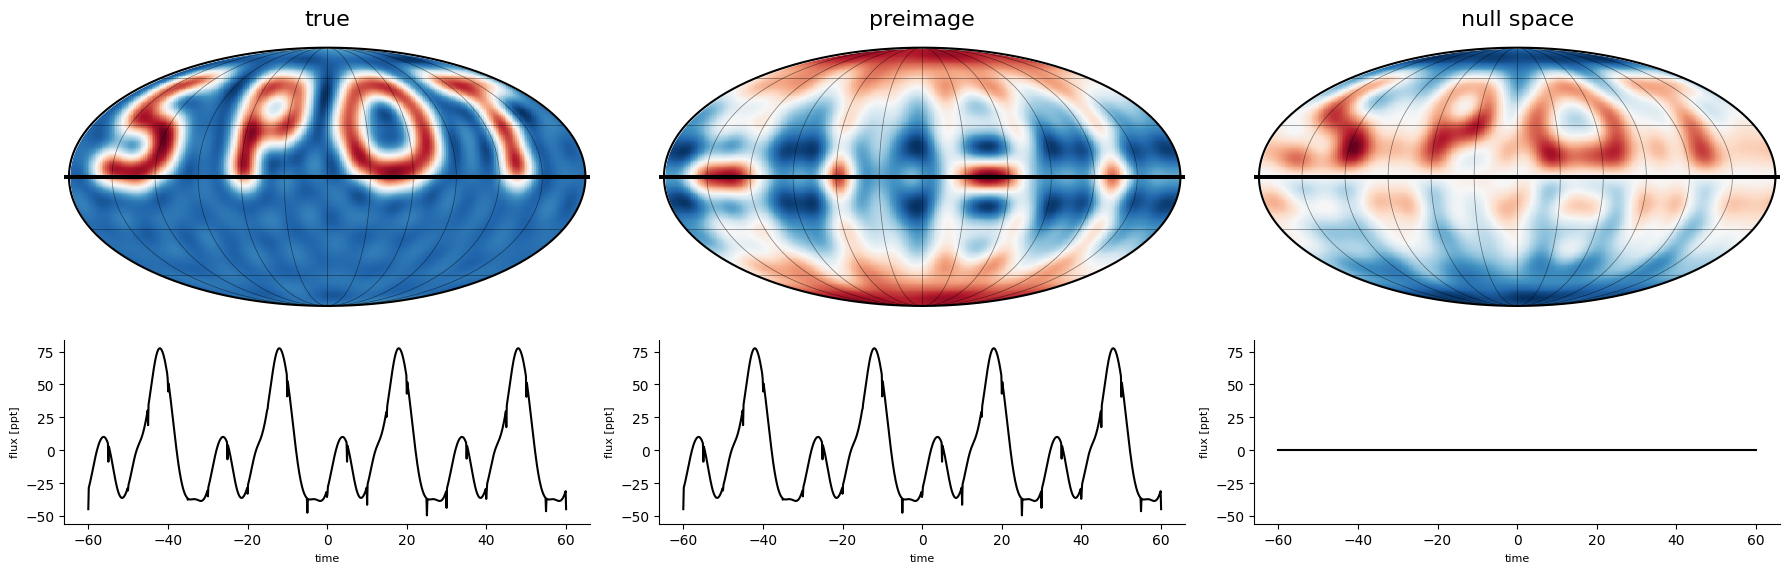
\includegraphics[width=\textwidth]{figures/nullspace-preimage.png}
        \caption{The breakdown of a surface map into its constituent components: the original map (left), its preimage (center), and null space (right). 
        Accompanying each set is the corresponding impact on the star's rotational light curve. The preimage represents surface patterns that 
        directly influence the observed light curve, while the null space encompasses patterns that have no effect on the flux measurements. 
        It's noteworthy that a significant portion of the surface features fall within the null space, meaning they do not contribute to the light curve 
        that we can observe and measure. The blck line shows the planetary trajectory, so what is important is that the preimage contains the full
        information under planetary trajectory, while the nullspace is missing it.}
        \label{fig:nullspace}
    \end{figure*}
% In this work, we develop a Gaussian process framework to model the surfaces of exoplanet-host stars based on time-series photometry. We utilize 
% expressive kernel function from \cite{Luger2021b}. We first use this model on a simulated data to test the model, then we apply the model to an active K-dwarf
% HAT-P-11. 

% The planet-hosting star HAT-P-11 has been extensively studied for its star spots. HAT-P-11 is orbited by a Neptune-sized exoplanet, HAT-P-11b, 
% which was discovered in 2008 via the transit method \citep{Bakos2010,Deming2011}. The transiting nature of HAT-P-11b has allowed for detailed 
% characterization of the star spot activity on HAT-P-11, as star spots that are occulted during the planet's transit cause detectable brightening in 
% the transit light curve \citep{Morris2017}. 


%
% \section{The Data}
% The data is collected by the \emph{Kepler} mission and we extracted it using
% \texttt{lightkurve}, a Python package for Kepler and TESS data analysis \citep{lightkurve}.
% %
% \begin{figure}[ht!]
%     \script{TransitFitsWithStarry.py}
%     \begin{centering}
%         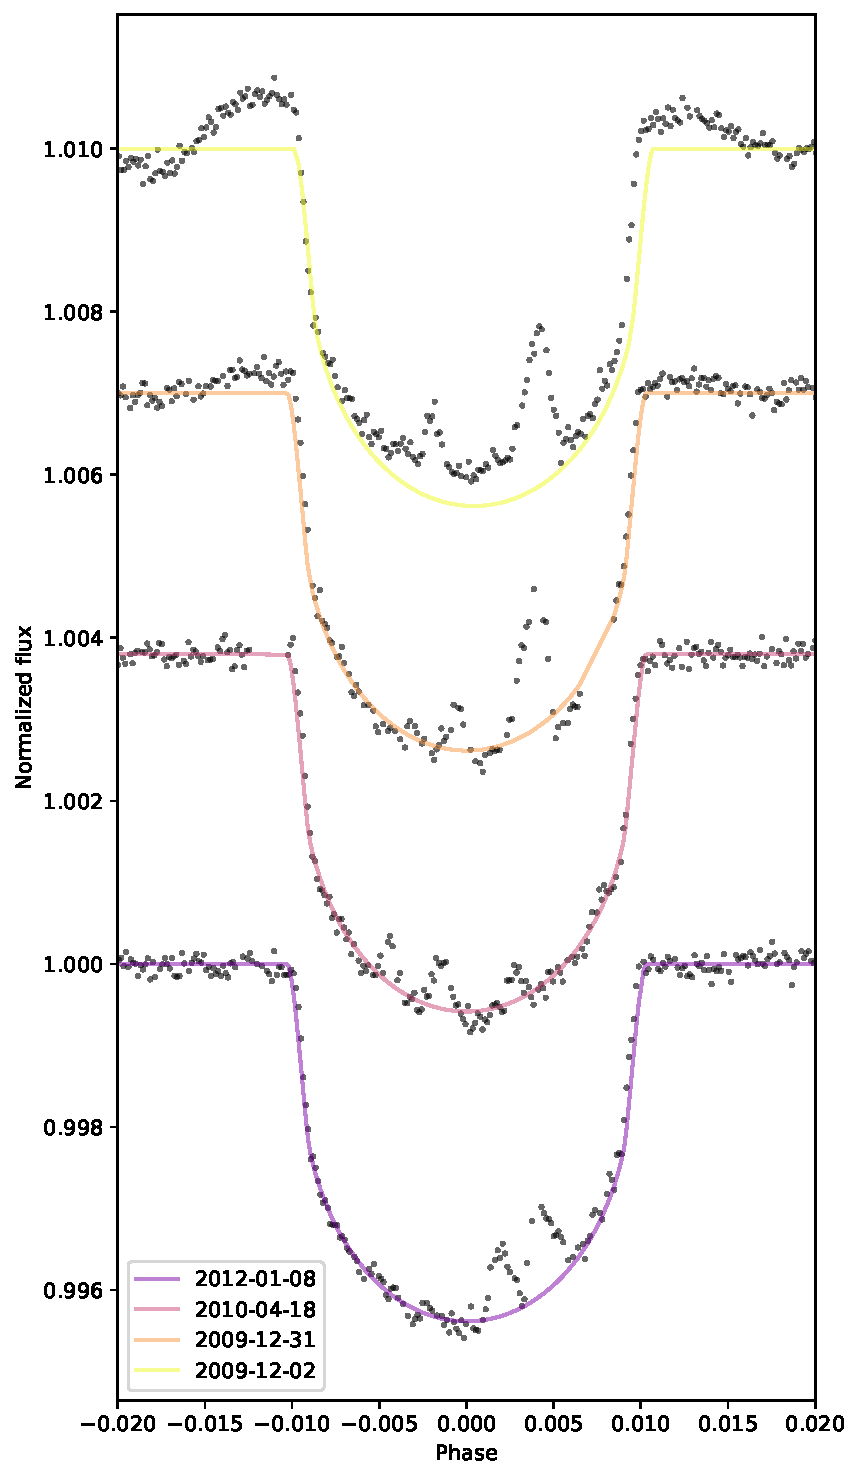
\includegraphics[width=\linewidth]{figures/TransitFitsWithStarry.pdf}
%         \caption{
%             Transit fits with starry -- no GPs.
%         }
%         \label{fig:TransitFitsStarry}
%     \end{centering}
% \end{figure}
%
\section{Hierarchical Bayesian model}
\label{sec:model}
In this section, we describe our Gaussian Process (GP) model and the likelihood calculation process used to estimate the model parameters.
This essentially means that we approximate the likelihood 
as a multidimensional Gaussian distribution characterized by a mean $\pmb{\mu}$ and covariance $\pmb{B}$ (for a comprehensive 
derivation of the Gaussian Process, refer to \cite{Luger2021b}):
%
\begin{align}
    \mathcal{L}\left(i_\star, P_\star, \mathbf{u}, \pmb{\theta}_\bullet\right) \sim
    \mathcal{N}\Big(
    \pmb{\mu}\left(i_\star, P_\star, \mathbf{u}, \pmb{\theta}_\bullet\right),
    \,
    \pmb{B}\left(i_\star, P_\star, \mathbf{u}, \pmb{\theta}_\bullet\right)
    \Big).
\end{align}
%
To infer the physical properties of the starposts, we want to obtain an underlying distribution of the physics conditioned on the provided data, 
which is known as the posterior distribution of the model.
% \subsection{Model for non-evolvng surfaces} \label{sec:nonevolmodel} 
We want to solve for a large set of parameters that includes the GP hyperparameters, the star's and the planet's orbital parameters, respectively. 
\begin{linenomath}\begin{align}
    \label{eq:largetheta}
    \pmb{\Theta}
     & =
    \left(
    \theta_\bullet
    \,\,\,
    \theta_\star
    \,\,\,
    \theta_p
    \right)^\top
    \quad,
\end{align}\end{linenomath}

Separately, these parameters are defined as 
\begin{linenomath}\begin{align}
    \label{eq:thetastar}
    \pmb{\theta_\star}
     & =
    \left(
    i_\star
    \,\,\,
    m_\star
    \,\,\,
    u_1
    \,\,\,
    u_2
    \,\,\,
    P_\star
    \right)^\top
    \quad,
\end{align}\end{linenomath}
where $i_\star$ is the star's orbital inclination, $m_\star$ is the stellar mass in the units of the solar mass, $u_1$ and $u_2$ are limb-darkening coefficients,
and $P_\star$ is the rotational period of the star.

\begin{linenomath}\begin{align}
    \label{eq:thetap}
    \pmb{\theta_p}
     & =
    \left(
    i_p
    \,\,\,
    e
    \,\,\,
    \lambda
    \,\,\,
    \omega
    \,\,\,
    P
    \,\,\,
    t_0
    \,\,\,
    R_p/R_\star
    \right)^\top
    \quad,
\end{align}\end{linenomath}
where $i_p$ is the planet's orbital inclination, $e$ is its eccenticity, $\lambda$ is the projected stellar obliquity, $\omega$ is the argument of pericenter of the planet,
$P$ is the rotational period of the planet, $t_0$ is the transit start time, and $R_p/R_\star$ is the planet to star radius ratio.

We represent the GP hyperparameters as \emph{physically interesting} set of parameters $\pmb{\theta}_\bullet$ \citep{Luger2021b}:
%
\begin{linenomath}\begin{align}
        \label{eq:thetaspot}
        \pmb{\theta}_\bullet
         & =
        \left(
        \mathbb{n}
        \,\,\,
        \mathbb{c}
        \,\,\,
        \mathbb{a}
        \,\,\,
        \mathbb{b}
        \,\,\,
        \mathbb{r}
        \right)^\top
        \quad,
    \end{align}\end{linenomath}
%
where $\mathbb{n}$ is the number of starspots, $\mathbb{c}$ is their contrast (defined as the intensity difference between the spot and the 
background intensity, as a fraction of the background intensity), and $\mathbb{r}$ is the radius
of the spots. $\mathbb{a}$ and $\mathbb{b}$ are the normalized parameters of the Beta distribution in $\cos\phi$, which is the probability density function (PDF) 
for the latitude $\phi$ of the spots. These parameters have a one-to-one correspondence to the mode $\mu_\phi$ and standard deviation $\sigma_\phi$ of the 
distribution in $\phi$, allowing for a concise representation of the latitudinal distribution characteristics.
The Beta distribution in $\cos\phi$ which has hyperparameters $\alpha$ and $\beta$, and the PDF given by
%
\begin{align}
    \label{eq:cosphi-pdf}
    p \big(\cos\phi \, \big| \, \alpha, \beta \big)
     & =
    \dfrac{\Gamma(\alpha + \beta)}{\Gamma(\alpha)\Gamma(\beta)}
    (\cos\phi)^{\alpha - 1}
    (1 - \cos\phi)^{\beta - 1}
    \quad,
\end{align}
%
where $\Gamma$ is the Gamma function. The $\alpha$ and $\beta$ are derived from the normalized parameters 
%
\begin{align}
    \label{eq:beta2gauss}
    \alpha & = \exp\left({K_{00} + (\ln\frac{1}{2})\mathbb{a}}\right)
    \nonumber                                                 \\
    \beta  & = \exp\left({\ln\frac{1}{2} + (10 - \ln\frac{1}{2})\mathbb{b}}\right)
    \quad,
\end{align}
%
with inverse transform
%
\begin{align}
    \label{eq:gauss2beta}
    \mathbb{a} & \equiv \frac{\ln\alpha}{\ln\frac{1}{2}}
    \nonumber                                             \\[0.5em]
    \mathbb{b} & \equiv \frac{\ln\beta - \ln\frac{1}{2}}{10 -\ln\frac{1}{2}}
\end{align}
%
The parameters $\mathbb{a}$ and $\mathbb{b}$ are both constrained to values between 0 and 1, making them convenient for sampling during the inference process. 
However, $\mathbb{a}$ and $\mathbb{b}$ do not have a straightforward relationship with physically meaningful quantities. In many situations, it is preferable to parametrize 
the latitude distribution using two parameters: $\mu_\phi$, which controls the central latitude, and $\sigma_\phi$, which governs the dispersion of the 
spots' latitudes. Here, both the mean $\mu_\phi$ and variance $\sigma^2_\phi$ can be derived from the Beta distribution as
%
\begin{align}
    \label{eq:mean_beta}
    \mu_\phi
     & =
    \dfrac{\alpha}{\alpha+\beta}
    \quad,
\end{align}
%
\begin{align}
    \label{eq:var_beta}
    \sigma^2_\phi
     & =
    \dfrac{\alpha\beta}{(\alpha+\beta)^2(\alpha+\beta+1)}
    \quad,
\end{align}
%

We assume that the prior over $\mathbb{f}_{true}$ follows a multivariate Gaussian distribution, with a mean vector of zeros and a covariance 
matrix $\pmb{B}$. We use the quasi-periodic kernel to define the covariance matrix $\pmb{B}$, which is defined by \texttt{StarryProcess}.
We assume that the observations $\mathbb{f}_{obs}$ are corrupted by additive Gaussian noise, such that:
\begin{equation}
    \mathbb{f}_{obs} = \mathbb{f}_{true} + \epsilon
\end{equation}

where $\epsilon \sim \mathcal{N}(0, \sigma_n^2)$ is the noise term. Given the GP prior and the likelihood function, we can 
calculate the joint posterior distribution over the hyperparameters $\Theta$ and the true function $\mathbb{f}_{true}$ given the observed data $\mathbb{f}_{obs}$:
%
\begin{equation}
    p(\Theta, \mathbb{f}_{true} \mid \mathbb{f}_{obs}) \propto p(\Theta) p(\mathbb{f}_{true} \mid \Theta) p(\mathbb{f}_{obs} \mid \mathbb{f}_{true})
\end{equation}
%
where $P(\Theta)$ is the prior distribution over the hyperparameters, $P(\mathbb{f}_{true} \mid \Theta)$ is the likelihood of the true function given 
the hyperparameters, and $P(f_{obs} \mid f_{true})$ is the likelihood of the observed data given the true function.
We calculate the log-likelihood function, given by (\citep{Luger2021b}):
%
% \begin{linenomath}\begin{align}
%     \label{eq:log-likeSabina}
%     \ln p(\mathbb{f}_{obs} \mid \pmb{\Theta}) 
%     =
%     & -\frac{1}{2} (\mathbb{f}_{obs} - \pmb{\mu})^T \pmb{B}^{-1} (\mathbb{f}_{obs} - \pmb{\mu}) 
%     \nonumber       \\[0.75em]
%     & -
%     \frac{1}{2} \ln |\pmb{B}| - \frac{n}{2} \ln (2\pi)
%     \quad,
% \end{align}\end{linenomath}
% %
% or, as defined in eq. 14 of \citep{Luger2021b}:
%
\begin{linenomath}\begin{align}
    \label{eq:log-likeRodrigo}
    \ln \mathcal{L}_m\left(\Theta\right)
    =
     & -\frac{1}{2}
    \mathbf{r}_m^\top\left(\Theta\right)
    \big[
        \pmb{B}\left(\Theta\right)
        \big]^{-1}
    \mathbf{r}_m\left(\Theta\right)
    \nonumber       \\[0.75em]
     & -
    \frac{1}{2}
    \ln \Big|
    \pmb{B}\left(\Theta\right)
    \Big|
    -
    \frac{K}{2}
    \ln \left( 2 \pi \right)
    \quad,
\end{align}\end{linenomath}
%
where
%
\begin{linenomath}\begin{align}
        \mathbf{r}_m\left(\pmb{\Theta}\right)
         & \equiv
        \mathbf{f}_m - \pmb{\mu}\left(\pmb{\Theta}\right)
    \end{align}\end{linenomath}
%
is defined as the residual vector,
%
$\pmb{B}$ is the full covariance, which is defined as 
%
\begin{linenomath}\begin{align}
    \pmb{B}\left(\Theta\right)
     & \equiv
    \pmb{\Lambda} + \pmb{C}
\end{align}\end{linenomath}
%
where $\pmb{\Lambda}$ is the covariance of the distribution over spherical harmonic coefficient
vectors $\mathbb{y}$, and $\pmb{C}$ is the data covariance, which is a diagonal
matrix whose entries are the squared uncertainty $\sigma_m^2$ corresponding to each data point in the light curve.
$| \cdots |$ denotes the determinant, and $K$ is the number of data points in
each light curve.%

For faster calculations we rewrite the likelihood function using \emph{the matrix conversion lemma}, also known as 
Woodbury-Sherman-Morrison identity (see, e.g., \cite{Hogg2020}), which gives an expression for the inverse $\pmb{B}^{-1}$ of the marginalized likelihood variance:
%
\begin{linenomath}\begin{align}
    \label{eq:Hoggtrick}
    \pmb{B}^{-1} = \pmb{C}^{-1} - \pmb{C}^{-1} \pmb{M} (\pmb{\mathbb{I}} 
    & + \pmb{\Lambda} \pmb{M}^T \pmb{C}^{-1}\pmb{M})^{-1}\pmb{\Lambda} \pmb{M}^T\pmb{C}^{-1}
\end{align}\end{linenomath}
%

% \section{Experiments}
% In this section, we describe the experiments we did on synthetic light curves before going ahead and modeling the real data. The synthetic light curves were 
% generated by initializing a planet and a star of similar parameters as HAT-P-11 b and HAT-P-11 have using \texttt{starry}. Then we draw \texttt{StarryProcess} 
% samples from a prior to get spherical harmonic coefficients and consequently the simulated flux. 

\subsection{The issue of the normalization of light curves and units}
Before going on discussing the experiments produced for this paper, we first need to remind the reader of a subtlety of the flux normalization when we are given
the raw light curves from telescopes. The problem and the ways to tackle it were described in \cite{Luger2021a} and \cite{Luger2021b}. 

Briefly, the problem of normalization of light curves is related to the fact that the observed flux from a star can vary due to a variety of factors 
such as atmospheric effects, instrumental noise, and changes in the intrinsic brightness of the star itself. These variations can make it difficult 
to compare light curves of different stars or even the same star observed at different times. To address this problem, astronomers typically normalize 
light curves by dividing the observed flux by some factor (the median or mean of the flux) that is assumed to be constant over time. 
However, as was described in \cite{Luger2021a}, if a star has a single large equatorial spot of contrast $c$ viewed at some high inclination 
(\cite{Luger2021a} used the value of $60^o$), and another star with a spot at the same location but with half the contrast \emph{and} a large polar spot of 
comparable contrast, then the light curves for both of the stars become indistiguishable in the relative units astronomers observe them. In addition to normalizing 
the flux, \cite{Luger2021a} also added a \emph{baseline} (1 in their case), which is the flux one would have gotten from a spotless star, 
and is an additive component to the $Y_m^l$.

In our experiments, we noticed that dividing by a constant factor \emph{and} adding an additive baseline messes up the units due to the 
intricate transition between the spherical harmonics and flux unit bases. To address this issue, we opt for an alternative approach, wherein we 
impose a constraint upon the constant terms within the map, which correspond to a featureless star. Specifically, we achieve this by setting the prior distribution 
over these constant terms to be entirely uniform, thereby setting the first row of the precision matrix to zero, which is us telling the model that
\textit{we don't know what the baseline is}.

Let $\mathbf{K}$ be the precision matrix, which is the inverse of the covariance matrix $\mathbf{B}$. Then the precision matrix looks as
%
\begin{linenomath}\begin{align}
    \mathbf{K} = 
    \begin{bmatrix}
    0 & 0 & \cdots & 0 \\
    0 & k_{22} & \cdots & k_{2n} \\
    \vdots & \vdots & \ddots & \vdots \\
    0 & k_{n2} & \cdots & k_{nn}
    \end{bmatrix}
\end{align}\end{linenomath}
%
where $k_{ij}$ represents the elements of the precision matrix $\mathbf{K}$.

By setting the first row of the precision matrix to zero, we effectively impose a uniform prior distribution over the constant terms in the map, thereby 
addressing the issue of unit mismatch caused by dividing by a constant factor and adding an additive baseline.

% In our experiments, we noticed that dividing by a constant factor \emph{and} adding an additive baseline messes up the units due to the complex change of 
% basis from spherical harmonics to the flux units. Instead, in our model, we set the baseline, i.e the first column of the design matrix, $\pmb{\mathcal{A}}$, 
% to have the coefficients of the 0th harmonic, $Y^0_0$ -- the featureless star. Then, the normalization "factor" becomes additive (not multiplicative!). We're reminding 
% the reader that $\pmb{\mathcal{A}}$ covers the properties of the star and the planet (inclination, rotation period, transit, etc.), spherical harmonics desribe the
% properties of the starspots. Therefore, what we get is
% %
% \begin{linenomath}\begin{align}
%         \label{eq:fAy}
%         \mathbf{f} = \pmb{\mathcal{a}_0(t)} \mathbf{y_0(t)} + \sum_{l=1, m=-l}^{15} \pmb{\mathcal{a}_{lm}(t)} \mathbf{y_{lm}(t)},
%     \end{align}\end{linenomath}
% %
% where $\pmb{\mathcal{a}_0}$ is a column of $\pmb{\mathcal{A}}(I, P, \mathbf{u})$, which is the design matrix as a function of the stellar inclination, rotation period, 
% and limb-darkening coefficients; $\mathbf{y}$ is a spherical harmonic coefficient vector, and we define $\pmb{\mathcal{a}_0} \mathbf{y_0} = \pmb{m}$ 
% as the normalization constant, or a \emph{baseline}. We explicitly solve for the baseline in our model. Note that it is not constant with time due to the transits --
% $\pmb{m}$ drops when the planet is transitting the star.

\subsection{Stellar inclination and obliquity}
\label{sec:obl-inc}
In the Sectrion \ref{sec:results-synthetic}, we hope to convince the reader that there is a a good amount of information about stars that we can learn 
from disk-integrated photometric measurements. In particular, Figure \ref{fig:inclination} illustrates the profound impact of stellar inclination on observed light curves. 
As the inclination angle varies from pole-on ($0^\circ$) to equator-on ($90^\circ$) views, we observe significant changes in both the amplitude and 
morphology of the light curve modulations. At low inclinations, when we view the star more pole-on, the light curves exhibit smaller amplitude variations. 
This is because the spots remain invisible throughout the stellar rotation, leading to more subtle flux changes. As the inclination increases towards an 
equator-on perspective, the amplitude of the variations typically increases, and the shape of the light curve becomes more pronounced. These changes occur because 
at higher inclinations, spots periodically disappear from view as the star rotates, causing more dramatic swings in the observed flux. 
The effect is particularly noticeable for spots at mid-latitudes, which can produce sharp dips in the light curve as they rotate into and out of view. 
It's important to note that while inclination significantly affects the observed light curve, it does not alter the underlying rotation period of 
the star or the intrinsic properties of the spots themselves.

While variations in stellar obliquity can have significant implications for planetary systems, their effects on the overall stellar light curve 
are often not noticeable. The global light curve is primarily influenced by the star's rotation and the distribution of spots on its surface, 
with obliquity playing a less prominent role. However, the impact of stellar obliquity becomes much more apparent during planetary transits, 
particularly through the phenomenon of spot-crossing events. When a planet transits its host star, it can occult starspots along its path. 
These spot-crossing events manifest as brief increases in brightness during the transit, as the planet temporarily blocks a darker region of the stellar 
surface. The frequency, timing, and duration of these spot-crossing events are strongly influenced by the alignment between the stellar spin axis and 
the planet's orbital plane - in other words, the stellar obliquity. Figure \ref{fig:obliquity} shows three consecutive transit light curves for 
different stellar obliquities. Each row in the figure represents a different obliquity scenario, with obliquity increasing from left to right. 
The rows display three consecutive transits for each scenario. 
In systems with low obliquity, where the stellar equator is aligned with the 
planet's orbit, spot-crossing events tend to occur more regularly and predictably. This is evident in the first column of Figure \ref{fig:obliquity}, where the spot-crossing patterns show a more consistent appearance across consecutive transits. 
Conversely, in systems with high obliquity, the pattern of spot-crossings can be more erratic and less frequent. This is because the planet's transit path across 
the stellar disk intersects a different range of stellar latitudes, potentially missing spots concentrated at certain latitudes. The $90^\circ$ column of 
Figure \ref{fig:obliquity} demonstrates this, showing more varied and less predictable spot-crossing patterns between consecutive transits. 
Therefore, while the full-disk light curve may not clearly reveal changes in stellar obliquity, careful analysis of in-transit light curves, 
particularly focusing on spot-crossing events, can provide valuable insights into the star's orientation relative to the planetary orbit. 

\begin{figure*}[hbt!]
    % \script{experiment-1-true-map.py}
    \begin{centering}
        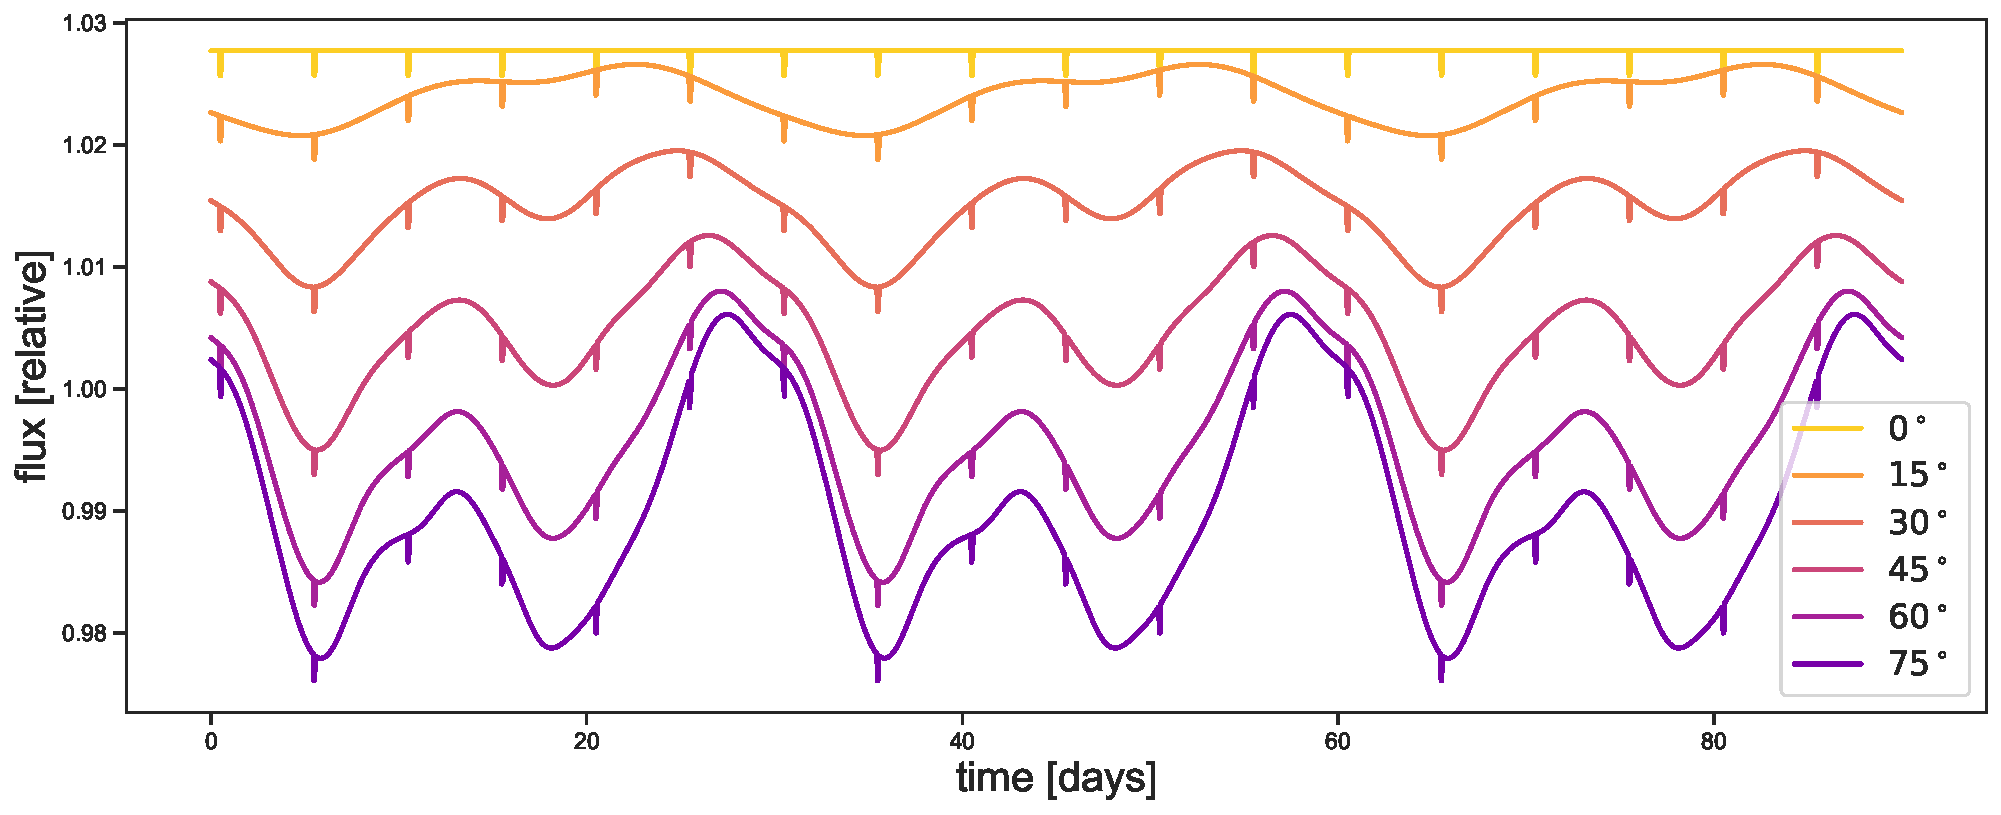
\includegraphics[width=\linewidth]{figures/inclinations.pdf}
        \caption{
            Variation in stellar light curves as a function of inclination angle. Each curve displays the photometric time series (light curve) for a 
            hypothetical spotted star observed at different inclination angles. The x-axis represents time in days, while the y-axis shows the relative flux. 
            Inclination angles range from $0^\circ$ (pole-on view) to $90^\circ$ (equator-on view). Note how the amplitude and shape of the light 
            curve modulations change significantly with inclination, demonstrating the importance of this parameter in interpreting stellar variability. 
            The star's rotation period and spot configuration remain constant across all light curves.
        }
        \label{fig:inclination}
    \end{centering}
\end{figure*}

\begin{figure*}[hbt!]
    % \script{experiment-1-true-map.py}
    \begin{centering}
        \includegraphics[width=\linewidth]{figures/obliquities.pdf}
        \caption{
            Impact of stellar obliquity on consecutive planetary transit light curves. Each column represents a different stellar obliquity scenario, 
            with obliquity increasing from left to right. The rows show three consecutive transits for each scenario. The x-axis represents time relative to 
            the transit center, while the y-axis shows the normalized flux. Note the varying patterns of in-transit brightness fluctuations 
            (spot-crossing events) across different obliquities and between consecutive transits. These differences arise from the changing 
            geometry between the planet's transit path and the distribution of starspots at different stellar latitudes. 
            The consistent transit depth and duration across all panels indicate that other system parameters remain constant, 
            isolating the effect of stellar obliquity.
        }
        \label{fig:obliquity}
    \end{centering}
\end{figure*}


While the analysis of spot-crossing events in transit light curves provides a powerful tool for constraining stellar inclination and obliquity, 
there exists an important degeneracy in these measurements. Specifically, a system with stellar inclination $i_\star$ and obliquity $-\lambda_\star$ 
will produce identical light curves to a system with inclination $180-i_\star$ and obliquity $\lambda_\star$, but with a surface map flipped upside down.

This degeneracy arises from the symmetry in the geometry of the star-planet system. In both scenarios, the relative orientation between the stellar 
rotation axis and the planet's orbital plane remains the same, merely mirrored. As a result, the pattern of spot crossings and their evolution over 
multiple transits will be indistinguishable between these two configurations.

For example, a star with an inclination of $80^\circ$ and an obliquity of $-30^\circ$ will present the same transit light curves 
as a star with an inclination of $100^\circ$ and an obliquity of $30^\circ$ with a flipped map (see Figure \ref{fig:inc-obliquity-degeneracy}). 
In both cases, the angle between the stellar spin axis and the planet's orbital axis is identical, just reflected about the plane of the sky.
This degeneracy highlights a limitation in our ability to uniquely determine stellar geometry solely from transit light curve analysis. 
While we can constrain the relative alignment between the stellar spin and planetary orbit with high precision, we cannot distinguish between these 
mirrored configurations without additional information or observations.


\begin{figure}[hbt!]
    % \script{experiment-1-true-map.py}
    \begin{centering}
        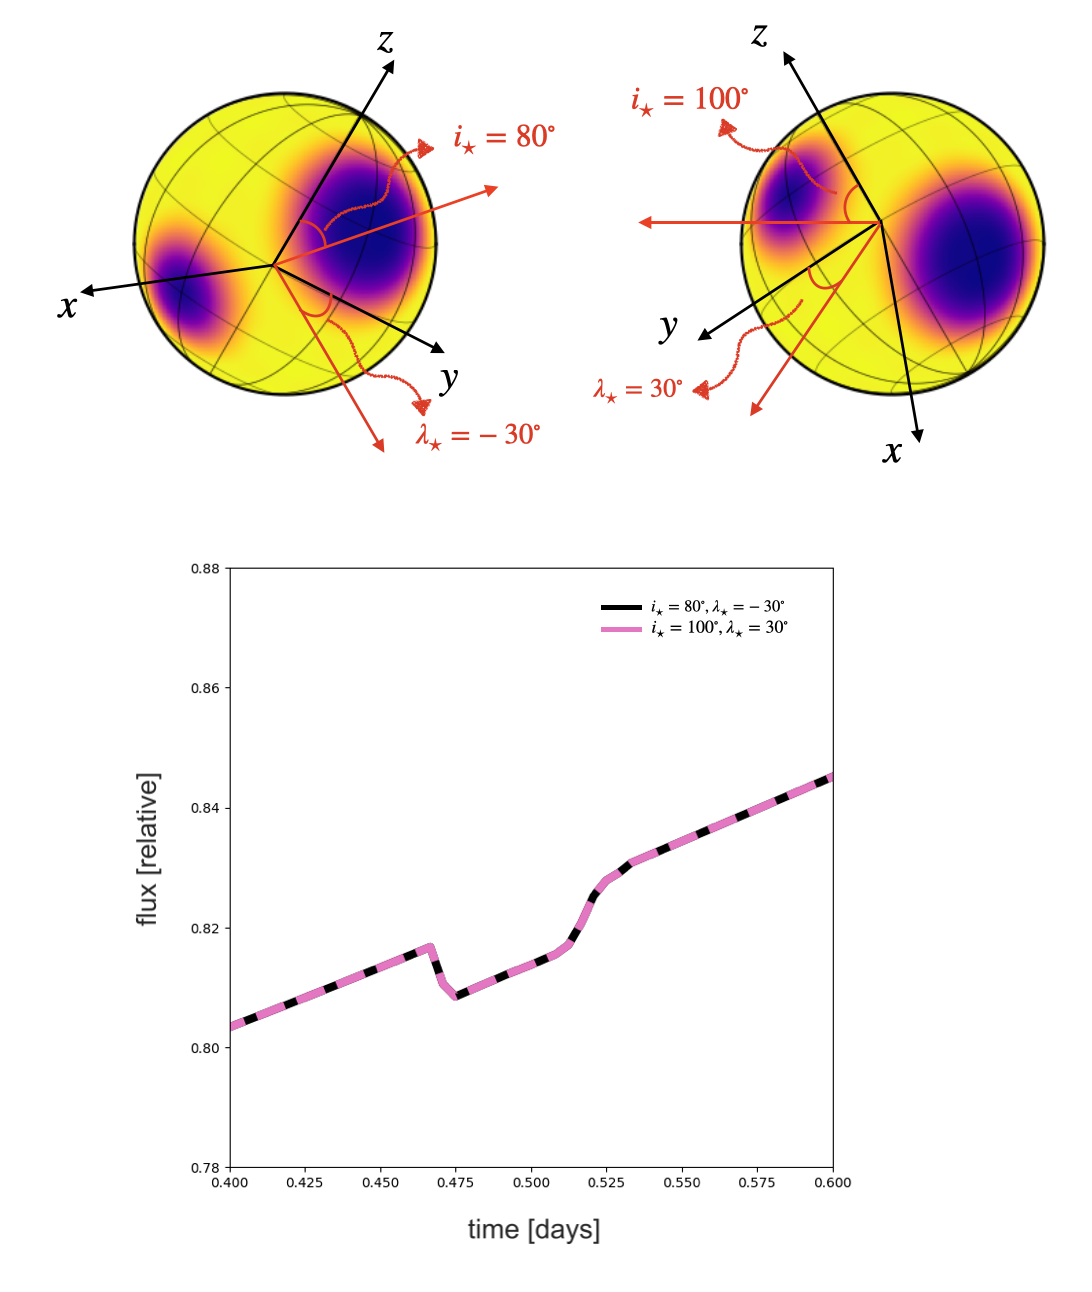
\includegraphics[width=\linewidth]{figures/inc-obl-degeneracy.png}
        \caption{
            Illustration of the degeneracy between stellar inclination ($i_\star$) and obliquity ($\lambda_\star$) in transit light curves. 
            The left panel shows a star-planet system with inclination $i_\star$ and obliquity $-\lambda_\star$, while the right panel 
            depicts a system with inclination $180-i_\star$ and obliquity $\lambda_\star$ and with a flipped map. 
            Despite the different geometries, both configurations result in identical transit light curves, shown in the central plot. 
            The x-axis represents time relative to the transit center, and the y-axis shows normalized flux. 
            This degeneracy demonstrates that while transit light curves can constrain the relative alignment between stellar spin and planetary orbit, 
            they cannot distinguish between these mirrored configurations without additional information. 
            The angles are represented with $x$, $y$, and $z$ vectors.
        }
        \label{fig:inc-obliquity-degeneracy}
    \end{centering}
\end{figure}

Given the degeneracy between stellar inclination and obliquity, a naive sampling approach could lead to unnecessary computational costs and potential 
convergence issues. To address this, we can leverage the fact that inclination and obliquity can be represented as vectors in three-dimensional 
space (see Figure \ref{fig:inc-obliquity-degeneracy}). This allows us to implement a more efficient sampling strategy that breaks the degeneracy 
while maintaining physical consistency.

We introduce transformed variables $\tilde{x}$, $\tilde{y}$, and $\tilde{z}$, on which we place prior distributions. 
Specifically, we use normal priors for $\tilde{x}$ and $\tilde{y}$, and a half-normal prior for $\tilde{z}$ to ensure it remains positive. 
These priors are chosen to explore the parameter space effectively while respecting physical constraints.

The transformation from these sampled variables to the physical space is then defined as:
\begin{linenomath}\begin{align}
    \label{eq:xyz}
    x = \tilde{x}, \\ 
    y = \frac{\sqrt{2}}{2} (\tilde{z} + \tilde{y}), \\
    z = \frac{\sqrt{2}}{2} (\tilde{z} - \tilde{y})
\end{align}\end{linenomath}

From these transformed coordinates, we can derive the stellar inclination and obliquity:

\begin{linenomath}\begin{align}
    \label{eq:obl-inc}
    i_\star = \arctan{\frac{y}{x}}, \\ 
    \lambda_\star = \arccos{\frac{z}{\sqrt{x^2 + y^2 + z^2}}}
\end{align}\end{linenomath}

This approach effectively breaks the degeneracy during the sampling process. By sampling in this transformed space and then mapping back to 
the physical parameters, we ensure that our model explores the full range of physically meaningful configurations without redundancy. 
This not only improves the efficiency of our sampling but also provides unambiguous constraints on the stellar geometry.

\subsection{Step-by-step model instruction}
In this section, we provide a comprehensive, step-by-step description of our model's methodology. 
This process outlines the key stages in our analysis, from initial data preparation to the final likelihood computation:

\begin{enumerate}
    \item Acquire the target system's light curve data.
    \item Preprocess the data by binning the out-of-transit observations to optimize computational efficiency while preserving signal fidelity.
    \item Construct a design matrix incorporating both planetary (transit) and stellar orbital parameters, encapsulating the geometry of the star-planet system.
    \item Establish physically motivated hyperparameters and prior distributions based on current astrophysical understanding and observational constraints.
    \item Implement a sampling algorithm to draw from the defined prior distributions, exploring the parameter space efficiently.
    \item Generate synthetic light curves from the sampled parameters, simulating the observed stellar and planetary signals.
    \item Compute the covariance matrix for the Gaussian process, which models the stochastic components of stellar variability.
    \item Assemble the inverse of the full covariance matrix, combining deterministic and stochastic elements of the model based on Equation \ref{eq:Hoggtrick}.
    \item Calculate the likelihood of the observed data given the model parameters, quantifying the agreement between our model and the observations with Equation \ref{eq:log-likeRodrigo}.
\end{enumerate}

\subsection{Model for evolving surfaces}
\label{sec:evolmodel}
Some active stars, particularly Sun-like stars, exhibit surface evolution on timescales as short as a single rotation period. For example, starspots can appear and dissipate within days or weeks, 
while chromospheric plages and coronal loops can flare up and decay on even shorter timescales. Such rapid evolution of surface structures violates 
the fundamental assumption of a static photosphere underlying the model described in Section \ref{sec:model}. 
Accounting for these time-dependent surface phenomena is crucial for accurately interpreting observations of active stars, as they can introduce significant 
time-varying distortions in the photometric light curves. 

Here, we describe an improved model that accounts for the surface evolution.

To account for the time-varying nature of the stellar surface maps, we have extended the model described in Section \ref{sec:model} to allow 
for a smooth evolution of the maps over time. We assume that the surface map transitions smoothly from one epoch to the next, with the spherical harmonic 
coefficients linearly interpolated between consecutive map epochs. 

Specifically, let $\pmb{y}_1$, $\pmb{y}_2$, $\pmb{y}_3$, ... represent the spherical harmonic coefficient vectors describing the surface maps at a 
sequence of epochs $\pmb{t}_1$, $\pmb{t}_2$, $\pmb{t}_3$, ... For any time $\pmb{t}$ between two consecutive epochs $\pmb{t}_i$ and $\pmb{t}_{i+1}$, 
the coefficient vector $\pmb{y(t)}$ is obtained by linear interpolation:
\begin{linenomath}\begin{align}\label{linearinterp}
    \pmb{y(t)} = (1 - \alpha)\pmb{y}_i + \alpha\pmb{y}_{i+1},
\end{align}\end{linenomath}

where $\alpha = (\pmb{t} - \pmb{t}_i) / (\pmb{t}_{i+1} - \pmb{t}_i)$ is the linear interpolation factor between the epochs. 
This interpolation scheme ensures the surface map smoothly deforms from $\pmb{y}_i$ at time $\pmb{t}_i$ to $\pmb{y}_{i+1}$ at the next epoch $\pmb{t}_{i+1}$.

A key aspect is that each pair of consecutive maps $\pmb{y}_i$, $\pmb{y}_{i+1}$ is interpolated independently from other map pairs. 
Thus, $\pmb{y}_{i+1}$ does not depend on $\pmb{y}_{i-1}$, and $\pmb{y}_{i+2}$ is independent of $\pmb{y}_{i+1}$, allowing the model greater 
flexibility to fit arbitrary time variations. The framework developed for static maps in Section \ref{sec:model} is applied independently 
to each interpolated map $\pmb{y(t)}$, with the transition between maps governed by the linear interpolation above.

% \subsection{Experiment on a non-evolving star}
% For our initial experiment with minimal complexity, we created a synthetic light curve that involved a single planetary transit (therefore, 
% \emph{a short light curve}). Here, we examined two distinct sampling techniques: No-U-Turn Sampling (NUTS) using \texttt{pymc3} and Markov Chain Monte Carlo (MCMC) 
% using \texttt{emcee}. The MCMC technique exhibited a faster convergence rate of the walkers, despite the fact that it still required a significant amount of time.
% \subsection{Long light curves (multiple transits)}

% \begin{figure}[ht!]
%     \script{synthetic_data.py}
%     \begin{centering}
%         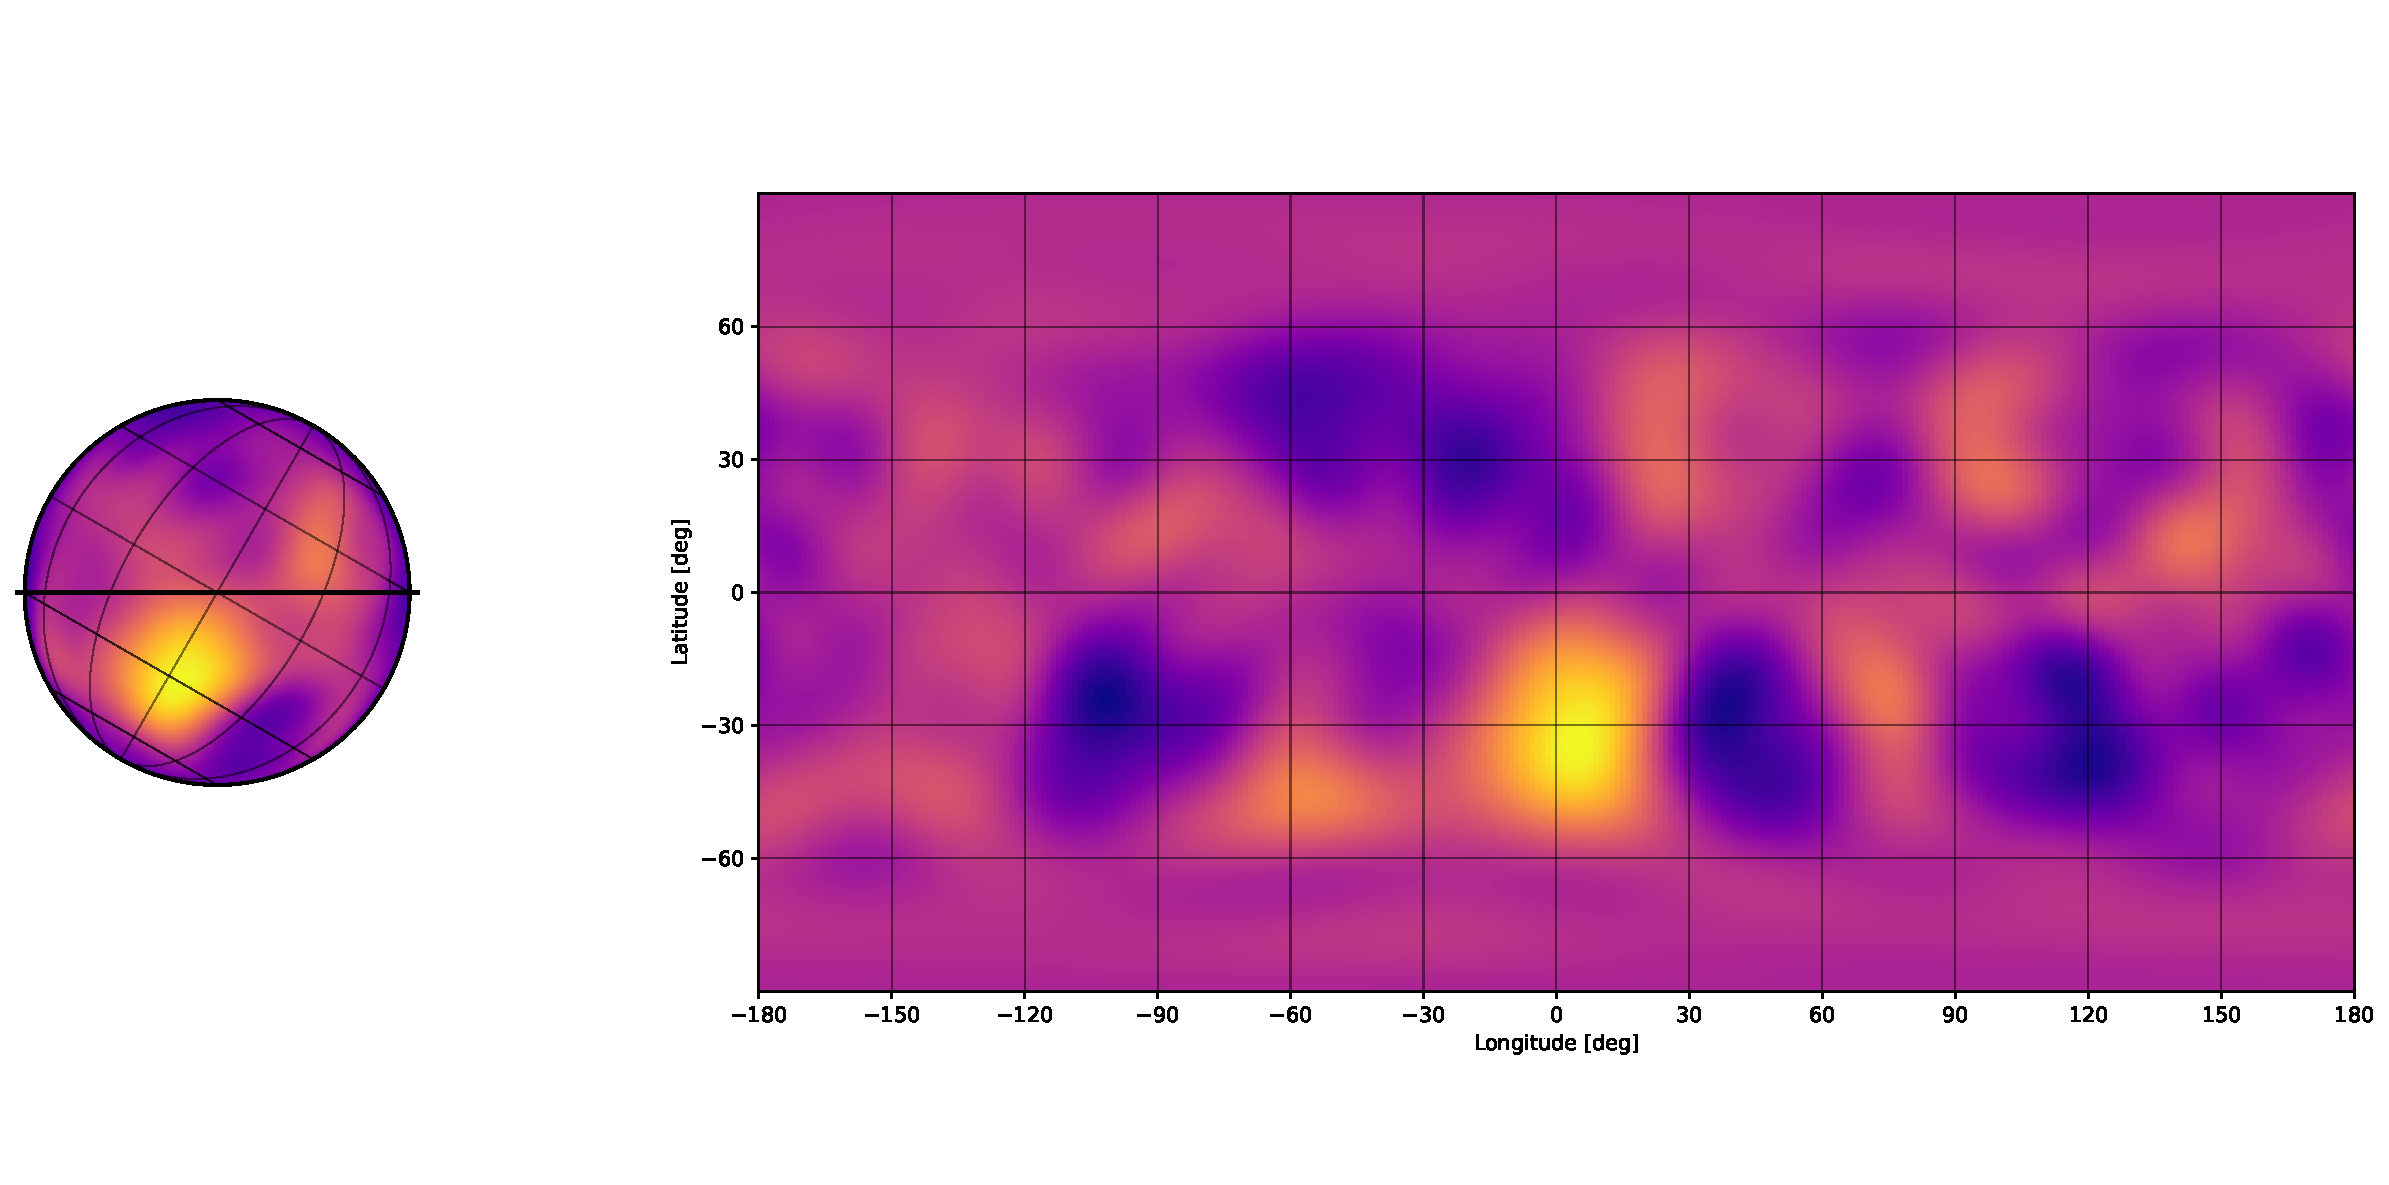
\includegraphics[width=\linewidth]{figures/SyntheticDataMap.pdf}
%         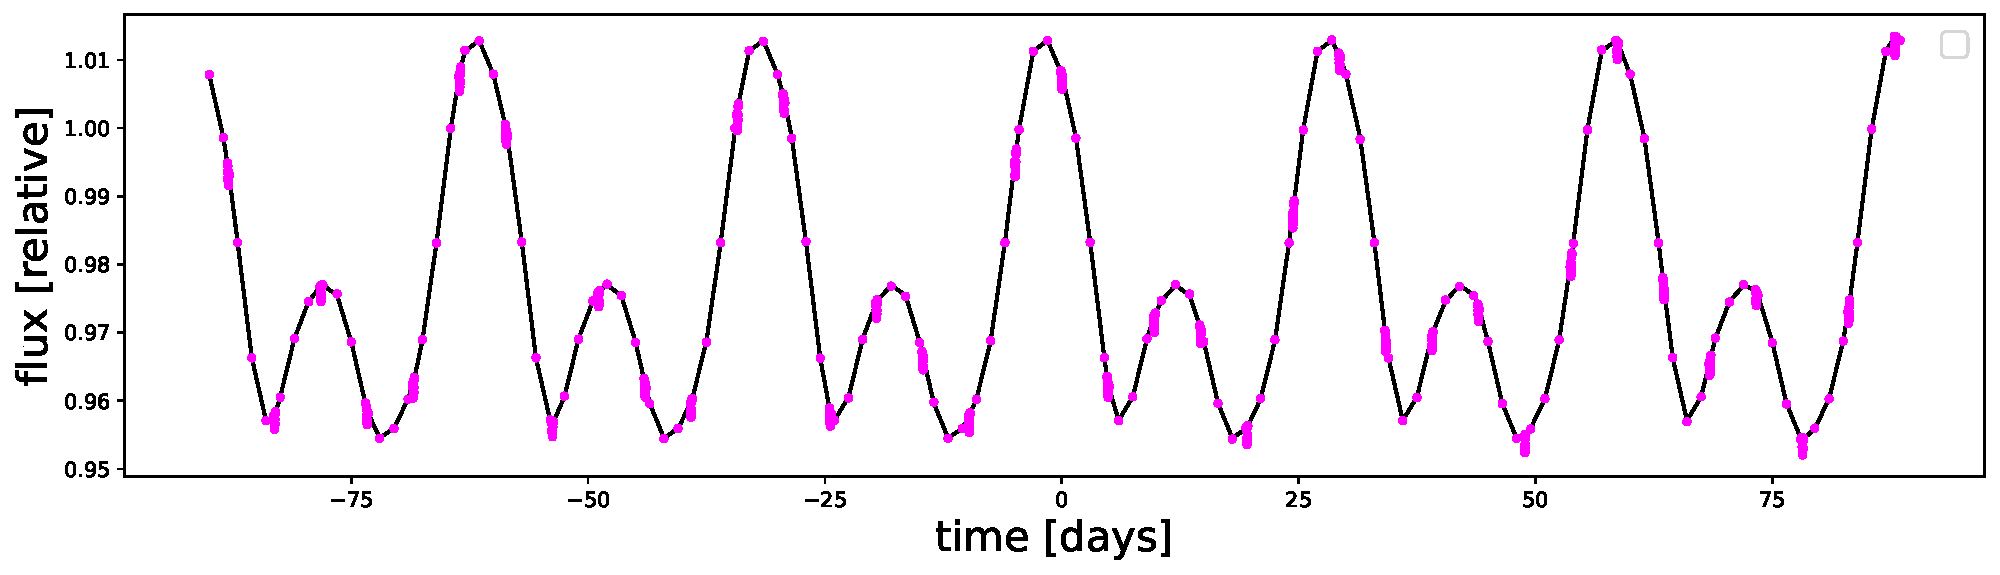
\includegraphics[width=\linewidth]{figures/SyntheticDataLightCurve.pdf}
%         \caption{
%             A synthetic dataset.
%         }
%         \label{fig:SyntheticDataLc}
%     \end{centering}
% \end{figure}

% \begin{figure}[ht!]
%     \script{synthetic_data.py}
%     \begin{centering}
%         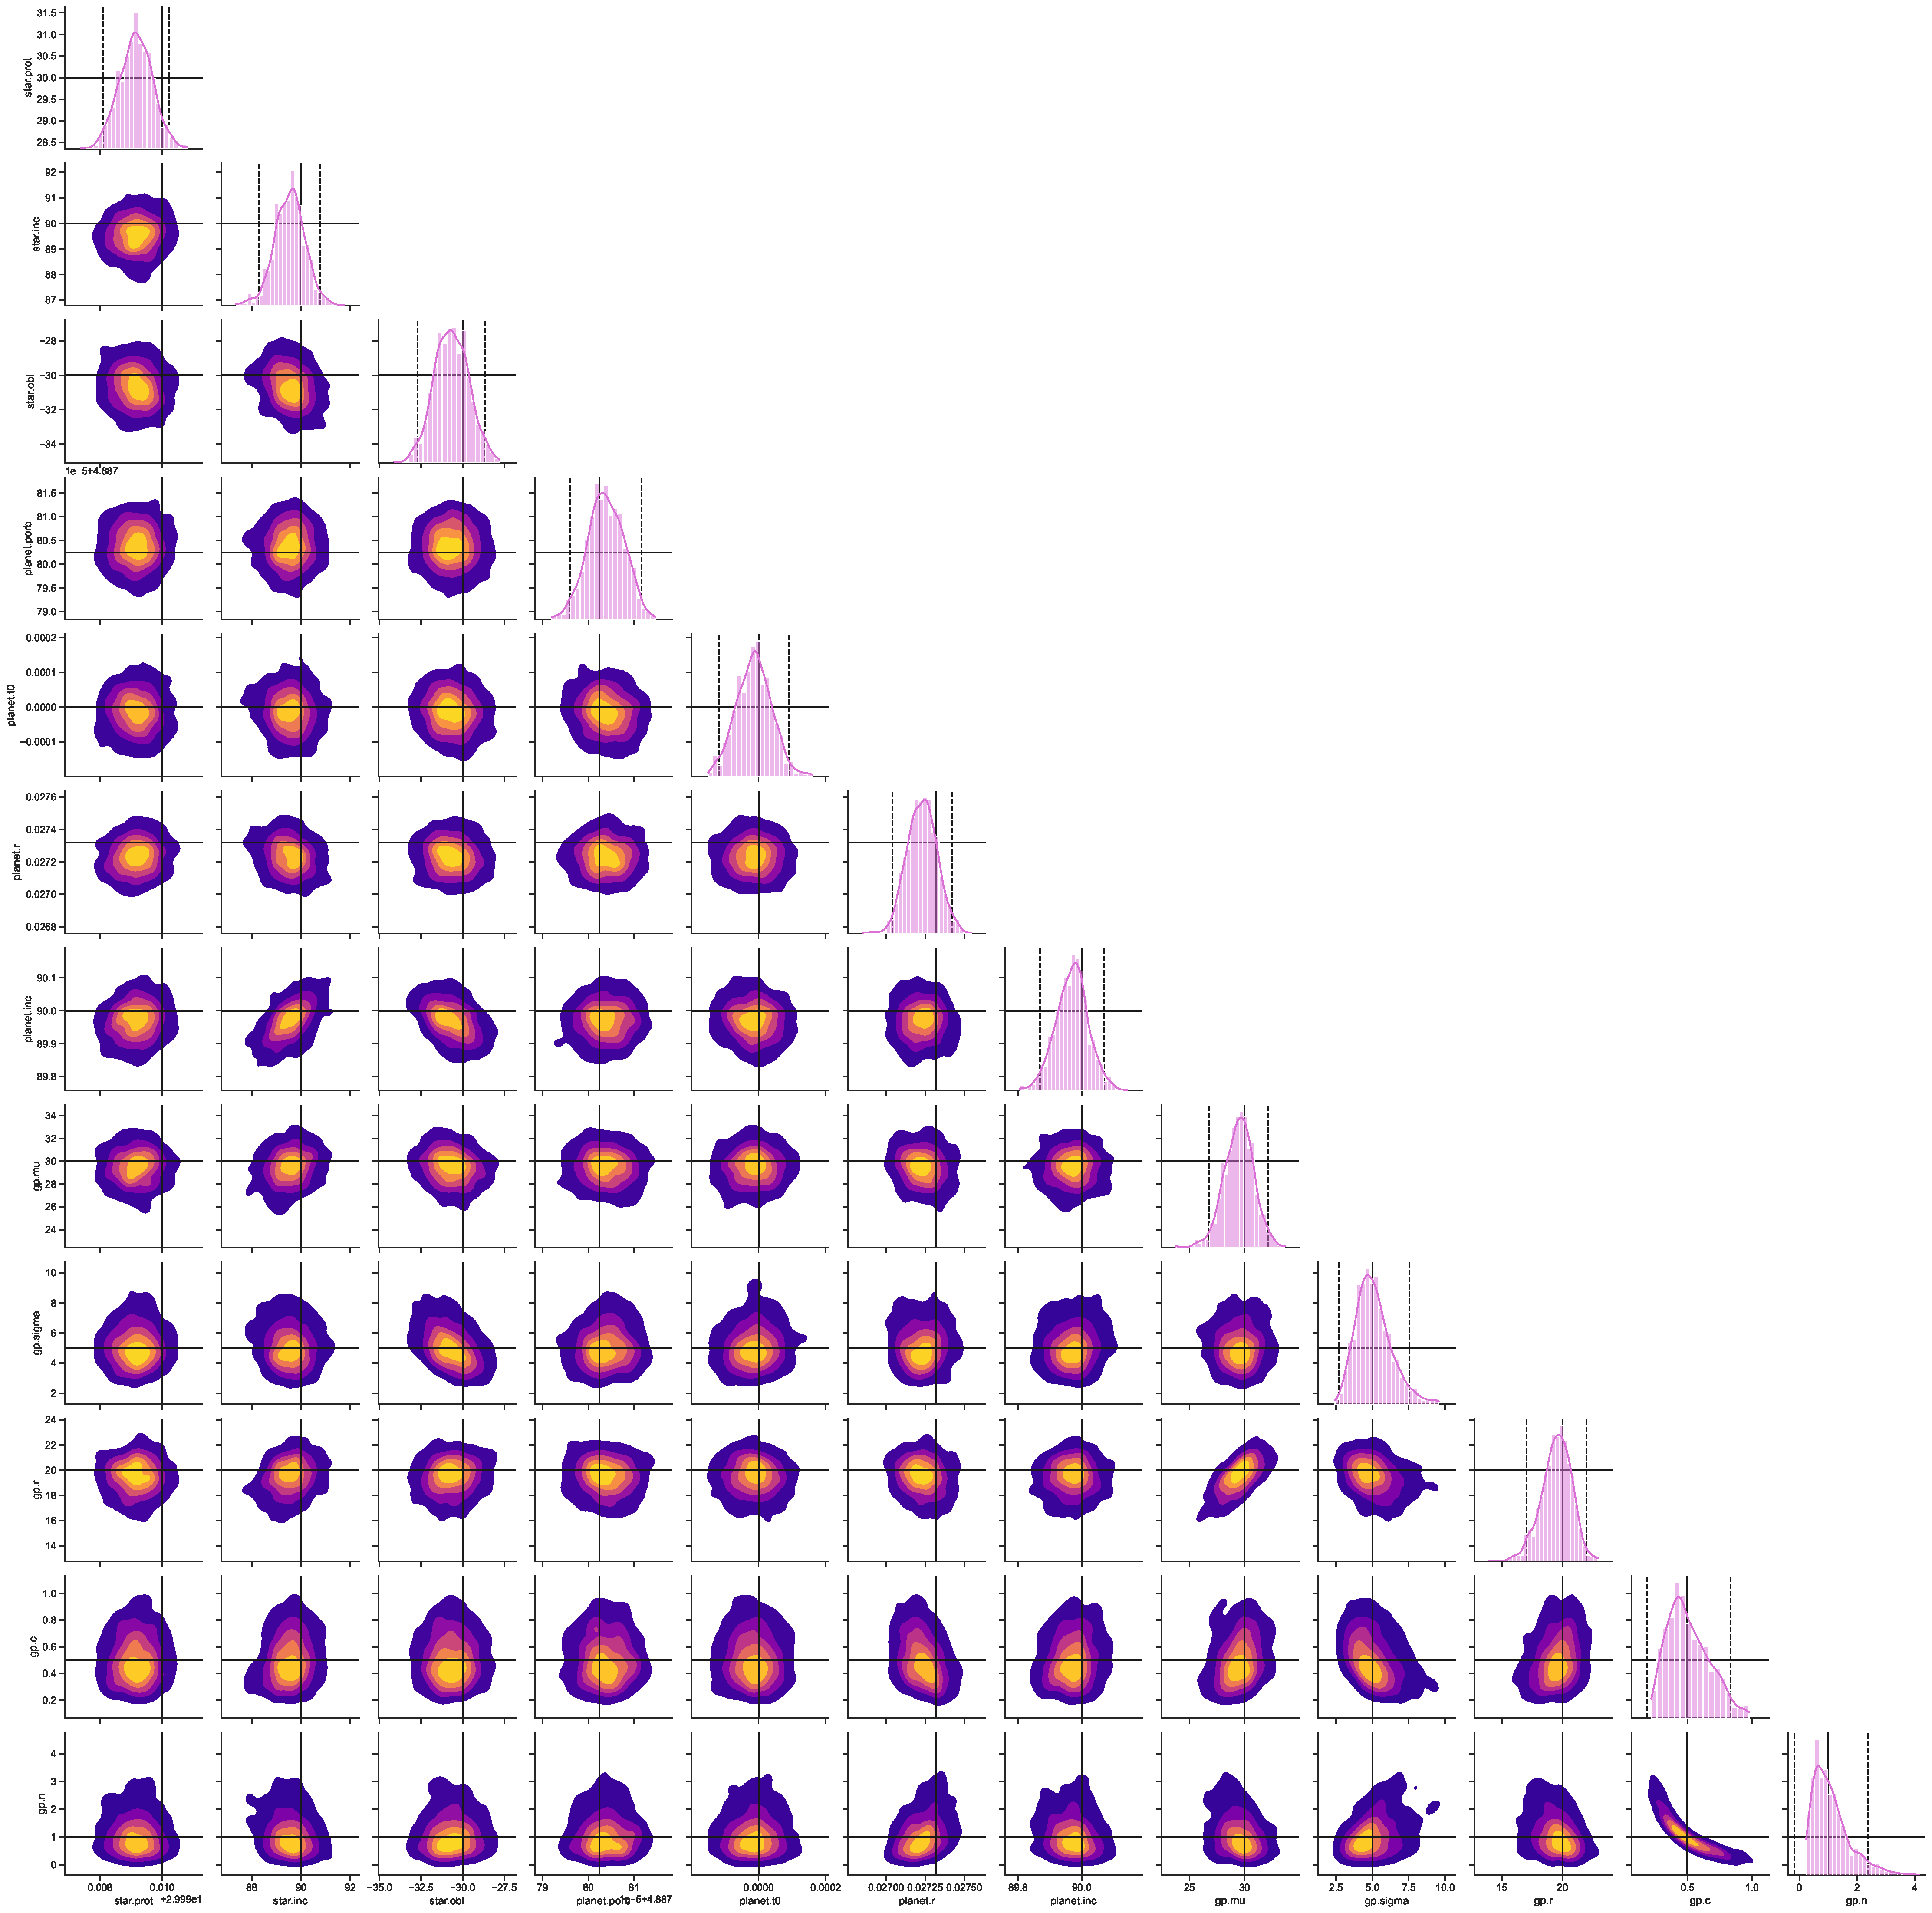
\includegraphics[width=\linewidth]{figures/SyntheticDataCorner.pdf}
%         \caption{
%             A synthetic dataset corner plot.
%         }
%         \label{fig:SyntheticDataCorner}
%     \end{centering}
% \end{figure}

\section{Results: synthetic datasets}
\label{sec:results-synthetic}
\subsection{Priors}
Before presenting the results, it is essential to elucidate the prior distributions employed throughout this work. 
We have implemented multiple priors in this work, carefully selected to maintain a balance between informativeness and generalizability. 
These priors serve to encapsulate our existing knowledge and assumptions about the parameters of interest, while allowing for sufficient flexibility 
to avoid computational cost.
\begin{itemize}
    \item $\sim\mathcal{U}(low, high)$: a uniform distribution.
    \item \textit{Planetary Inclination}: Considering that $i_p=\arccos{b}$, where $b$ is the impact parameter,
    the prior on the inclination is defined via the uniform prior $\sim\mathcal{U}(-b_{max}, -b_{max})$ on $b$, where $b_{max} = R_{\star} / a$.
    \item \textit{Period}: a prior on $P$ and $P_{\star}$. Instead of directly constraining the period, this prior works in log-space to ensure the period 
    remains positive and to make the distribution more symmetric. The actual prior is a uniform distribution in log-space, bounded by the log of the true 
    value plus or minus some fraction. The final period is determined by exponentiating the result of this log-uniform distribution, 
    which effectively creates a kind of log-uniform prior on the period itself.
    \item \textit{Logarithmic}: a log-uniform distribution.
    \item \textit{Stellar Angle}: a normal distribution on orientation vectors $\tilde{x}$ and $\tilde{y}$ and a half-normal distribution on $\tilde{z}$. See Section
    \ref{sec:obl-inc} for the full explanation.
\end{itemize}

\subsection{Experiment I: non-evolving surface}
\label{sec:experiment1}
To verify the proper calibration of our model, we evaluate its performance using synthetic data, which is created through the following process.
We create a system consisting of a star and a planet, each of them have some orbital parameters presented in Table \ref{tab:LongPriors}. 
The \textit{true} map is just a random draw from a from the process evaluated up to spherical harmonic degree
$l_{max} = 15$ and conditioned on different values of the hyperparameter vector $\pmb{\theta}_\bullet$ (Table \ref{tab:LongPriors}). Figure \ref{fig:experiment-1-map} 
illustrates the setup of Experiment I. The upper panel displays the "true" map used in the experiment, which represents the underlying reality that 
the model aims to reconstruct. This map represents the brightness distribution across the star's surface. We generated 90 days of observations with a 2-minute
cadence, and then we binned the out-of-transit flux to speed up the sampling process.
\begin{figure*}[ht!]
    % \script{experiment-1-true-map.py}
    \begin{centering}
        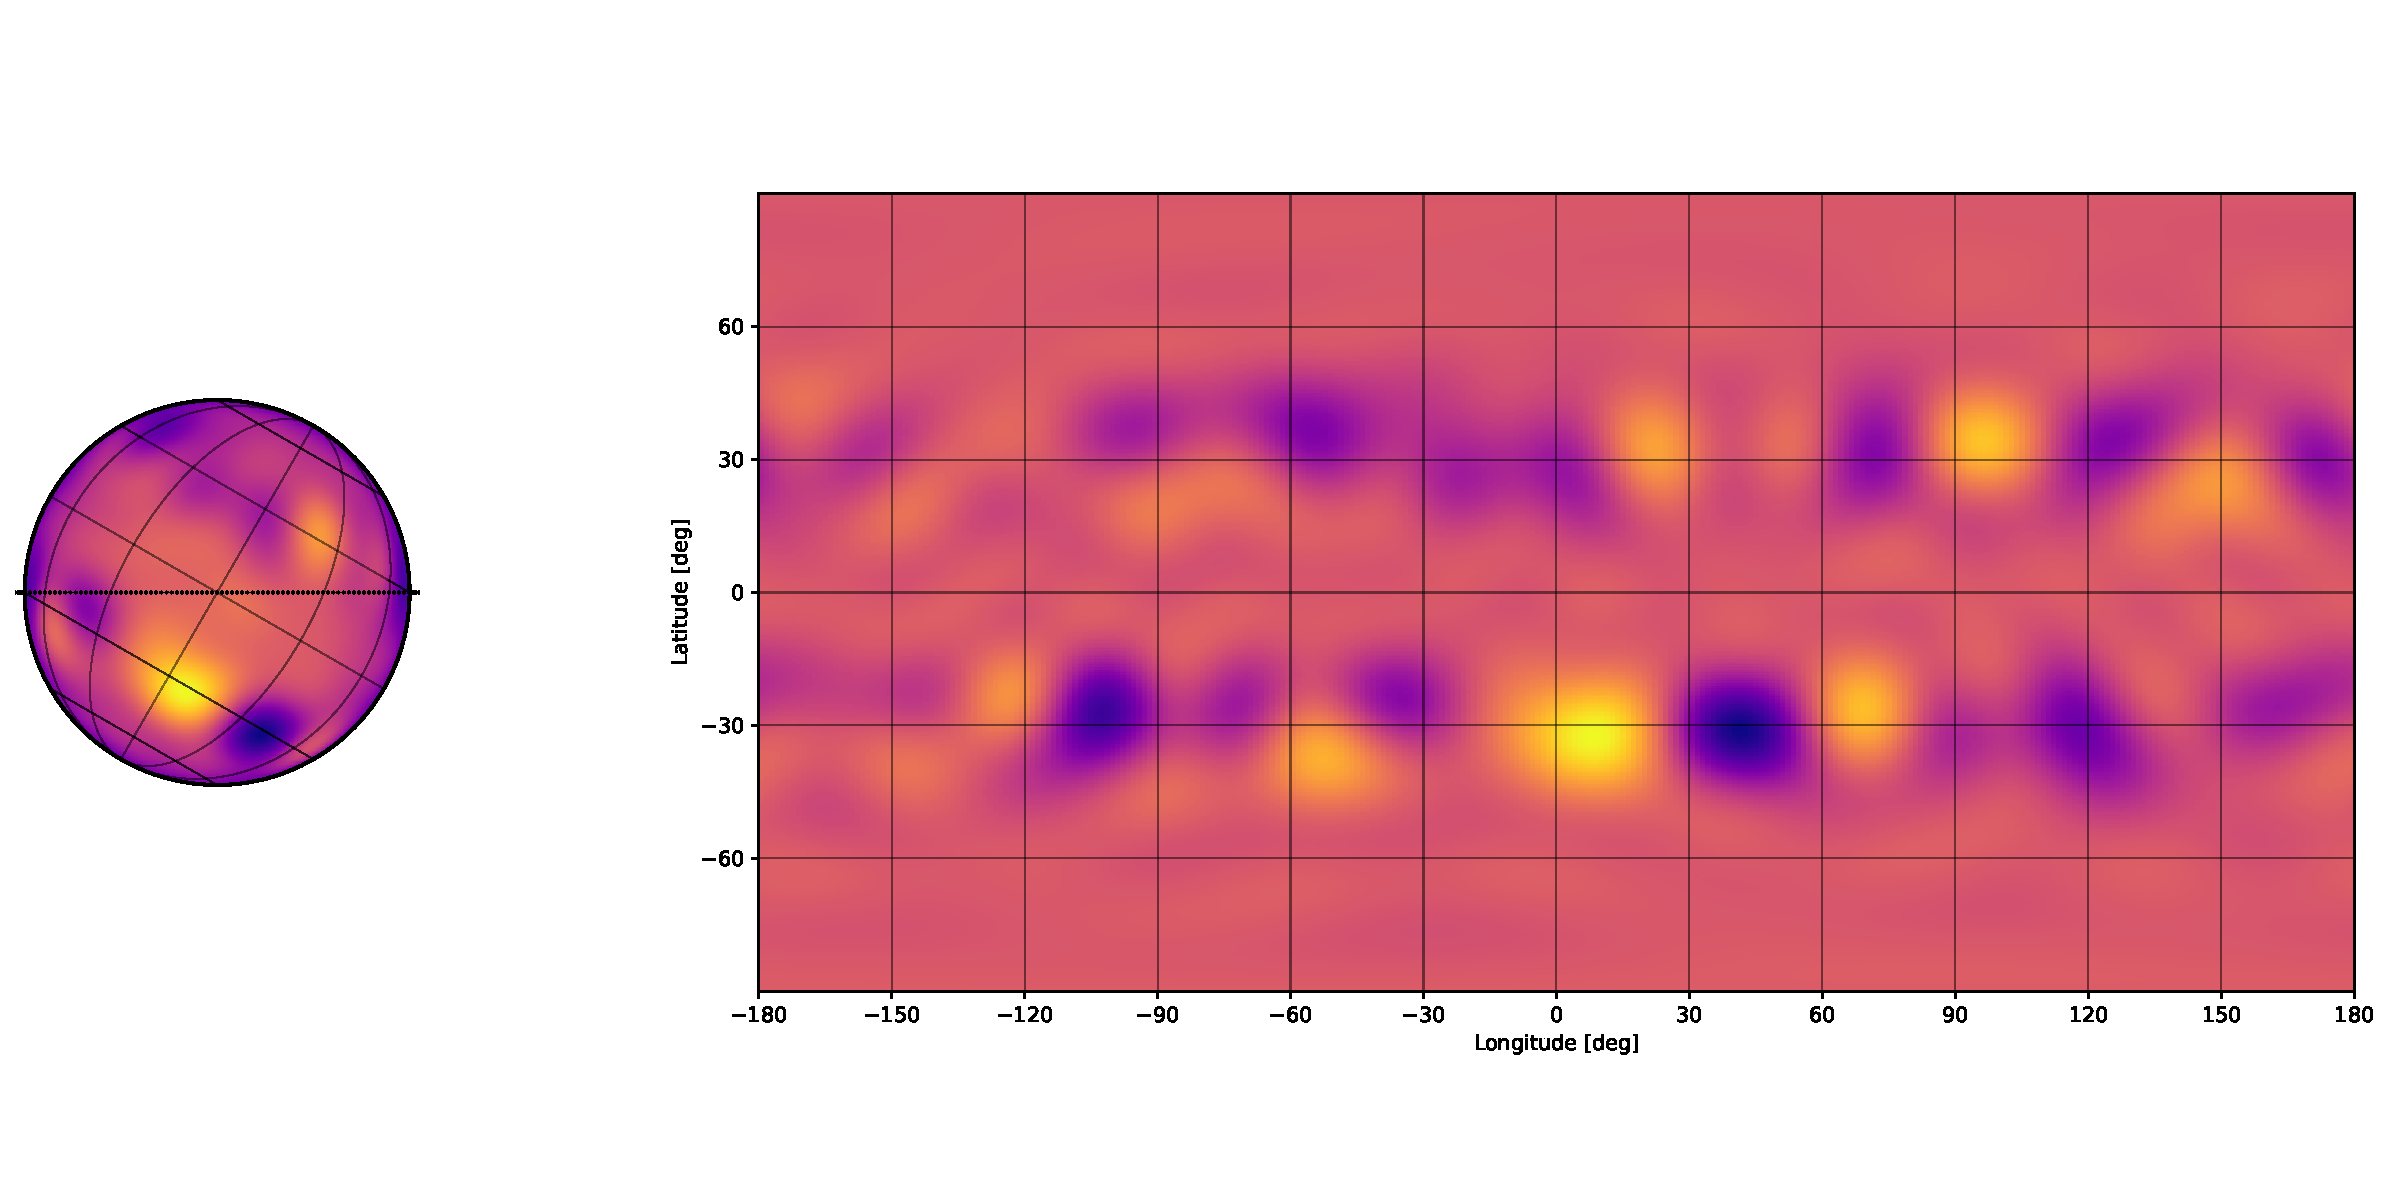
\includegraphics[width=\linewidth]{figures/experiment-1-true-map.pdf}
        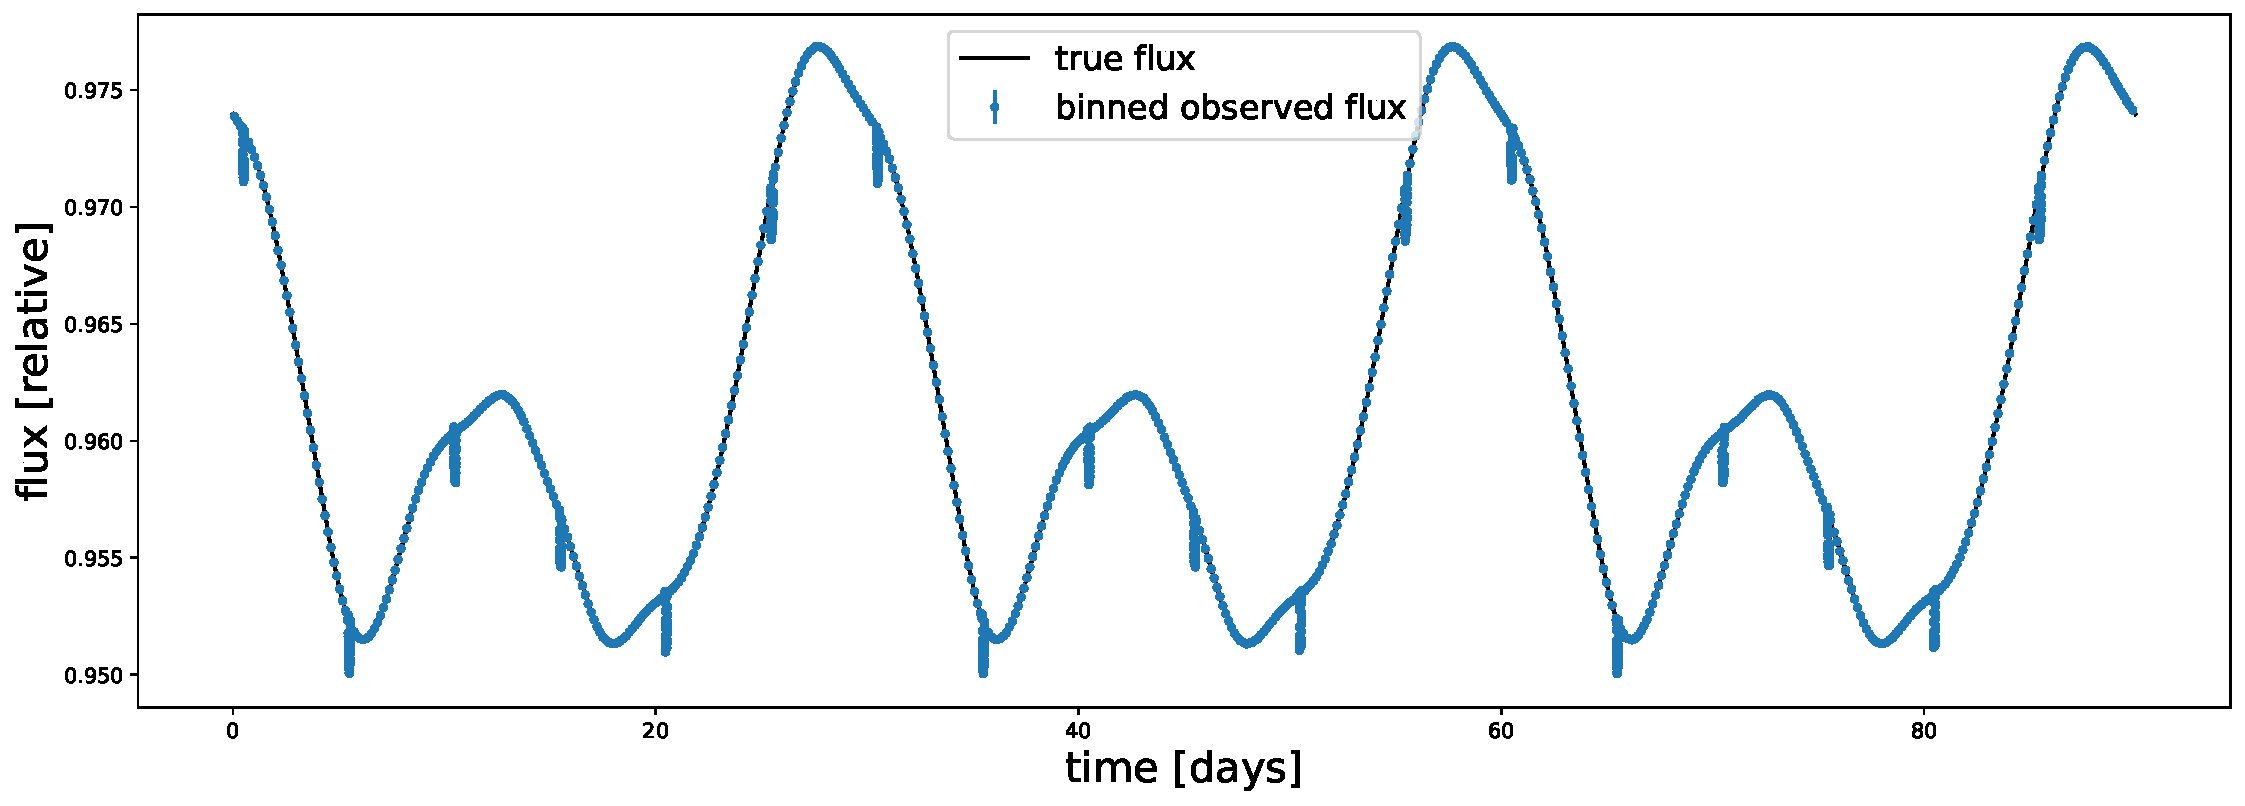
\includegraphics[width=\linewidth]{figures/experiment-1-lc.pdf}
        \caption{
            The upper panel shows the \textit{true} map for the Experiment I of this paper. The black dots on the map indicate the trajectory of the 
            planet as it moves across the face of the star during the transit event. The left panel 
            shows the stellar map along with its orientation on the sky and the right panel shows the rectangular projection of the map. 
            The bottom panel is the generated light curve. The black line is the \textit{true} light curve and the blue dots show the binned light curve
            that's used in the model.
        }
        \label{fig:experiment-1-map}
    \end{centering}
\end{figure*}

We utilized the \texttt{Python}-based implementation of the GP introduced by \cite{Luger2021b} to perform inference on the synthetic dataset. 
We used No-U-Turn Sampling, a variant of Hamiltonian Monte Carlo 
(NUTS; \cite{Duane1987,Hoffman2011}) to do posterior inference on our synthetic dataset.

We use several parameters in our sampling process: $i_p$ (the planetary inclination), $e$ (its eccentricity), $P$ (its orbital period),
$t_0$ (start of the transit time), $R_p/R_\star$ (ratio of planetary to stellar radius), $u_1$ and $u_2$ (limb darkening coefficients),
$i_\star$ (stellar inclination), $\lambda_\star$ (stellar obliquity), $P_\star$ (stellar rotational period), $\mathbb{n}$ (the number of spots), 
$\mathbb{c}$ (their contrast), $\mathbb{r}$ (their radius), and $\mathbb{a}$ and $\mathbb{b}$ (parameters of the Beta distribution that describe 
how the spots are spread across latitudes). As explained in \ref{sec:model}, it's more convenient to sample using $\mathbb{a}$ and $\mathbb{b}$ 
rather than the mean $\mu_\phi$  and standard deviation $\sigma^2_\phi$ of the latitude distribution. 
However, we transform $\mathbb{a}$ and $\mathbb{b}$ to posteriors in $\mu_\phi$  and $\sigma^2_\phi$ via Equations \ref{eq:beta2gauss}, 
\ref{eq:mean_beta}, \ref{eq:var_beta} and show the resuts with the parameters $\mu_\phi$ and $\sigma^2_\phi$ hence they are more intuitive for understanding. 

We use Equation \ref{eq:log-likeRodrigo} as our log likelihood term. The results are shown on Figure \ref{fig:experiment-1-map-corner-all},
where we correctly infer almost all five parameters within $\sim 2$ standard deviations. The only parameters that are not constrained too well are 
planetary eccentricity $e$ and the radius of spots $\mathbb{r}$, but they are still fairly close to the true values: the true value for the
eccenticity is 0.2 while the inferred median value is 0.225, and the true value for the radius of spots is $10^\circ$ while the inferred median value is
$14.3^\circ$. 

To visually demonstrate the performance of our model, Figure \ref{fig:experiment-1-map-comparison} presents a comprehensive comparison between 
the true stellar surface used in our synthetic data generation and the inferred surface map from our analysis, alongside the resulting light curve fit and 
transit details. Of particular interest are the three consecutive transits shown in detail on the right panel. These zoomed-in views highlight our 
model's ability to precisely fit transit events, including subtle spot-crossing phenomena. The spot-crossing events, visible as brief increases in brightness 
during the transits, are well-captured by our model.
%
\begin{figure*}[hbt!]
    % \script{experiment-1-true-map.py}
    \begin{centering}
        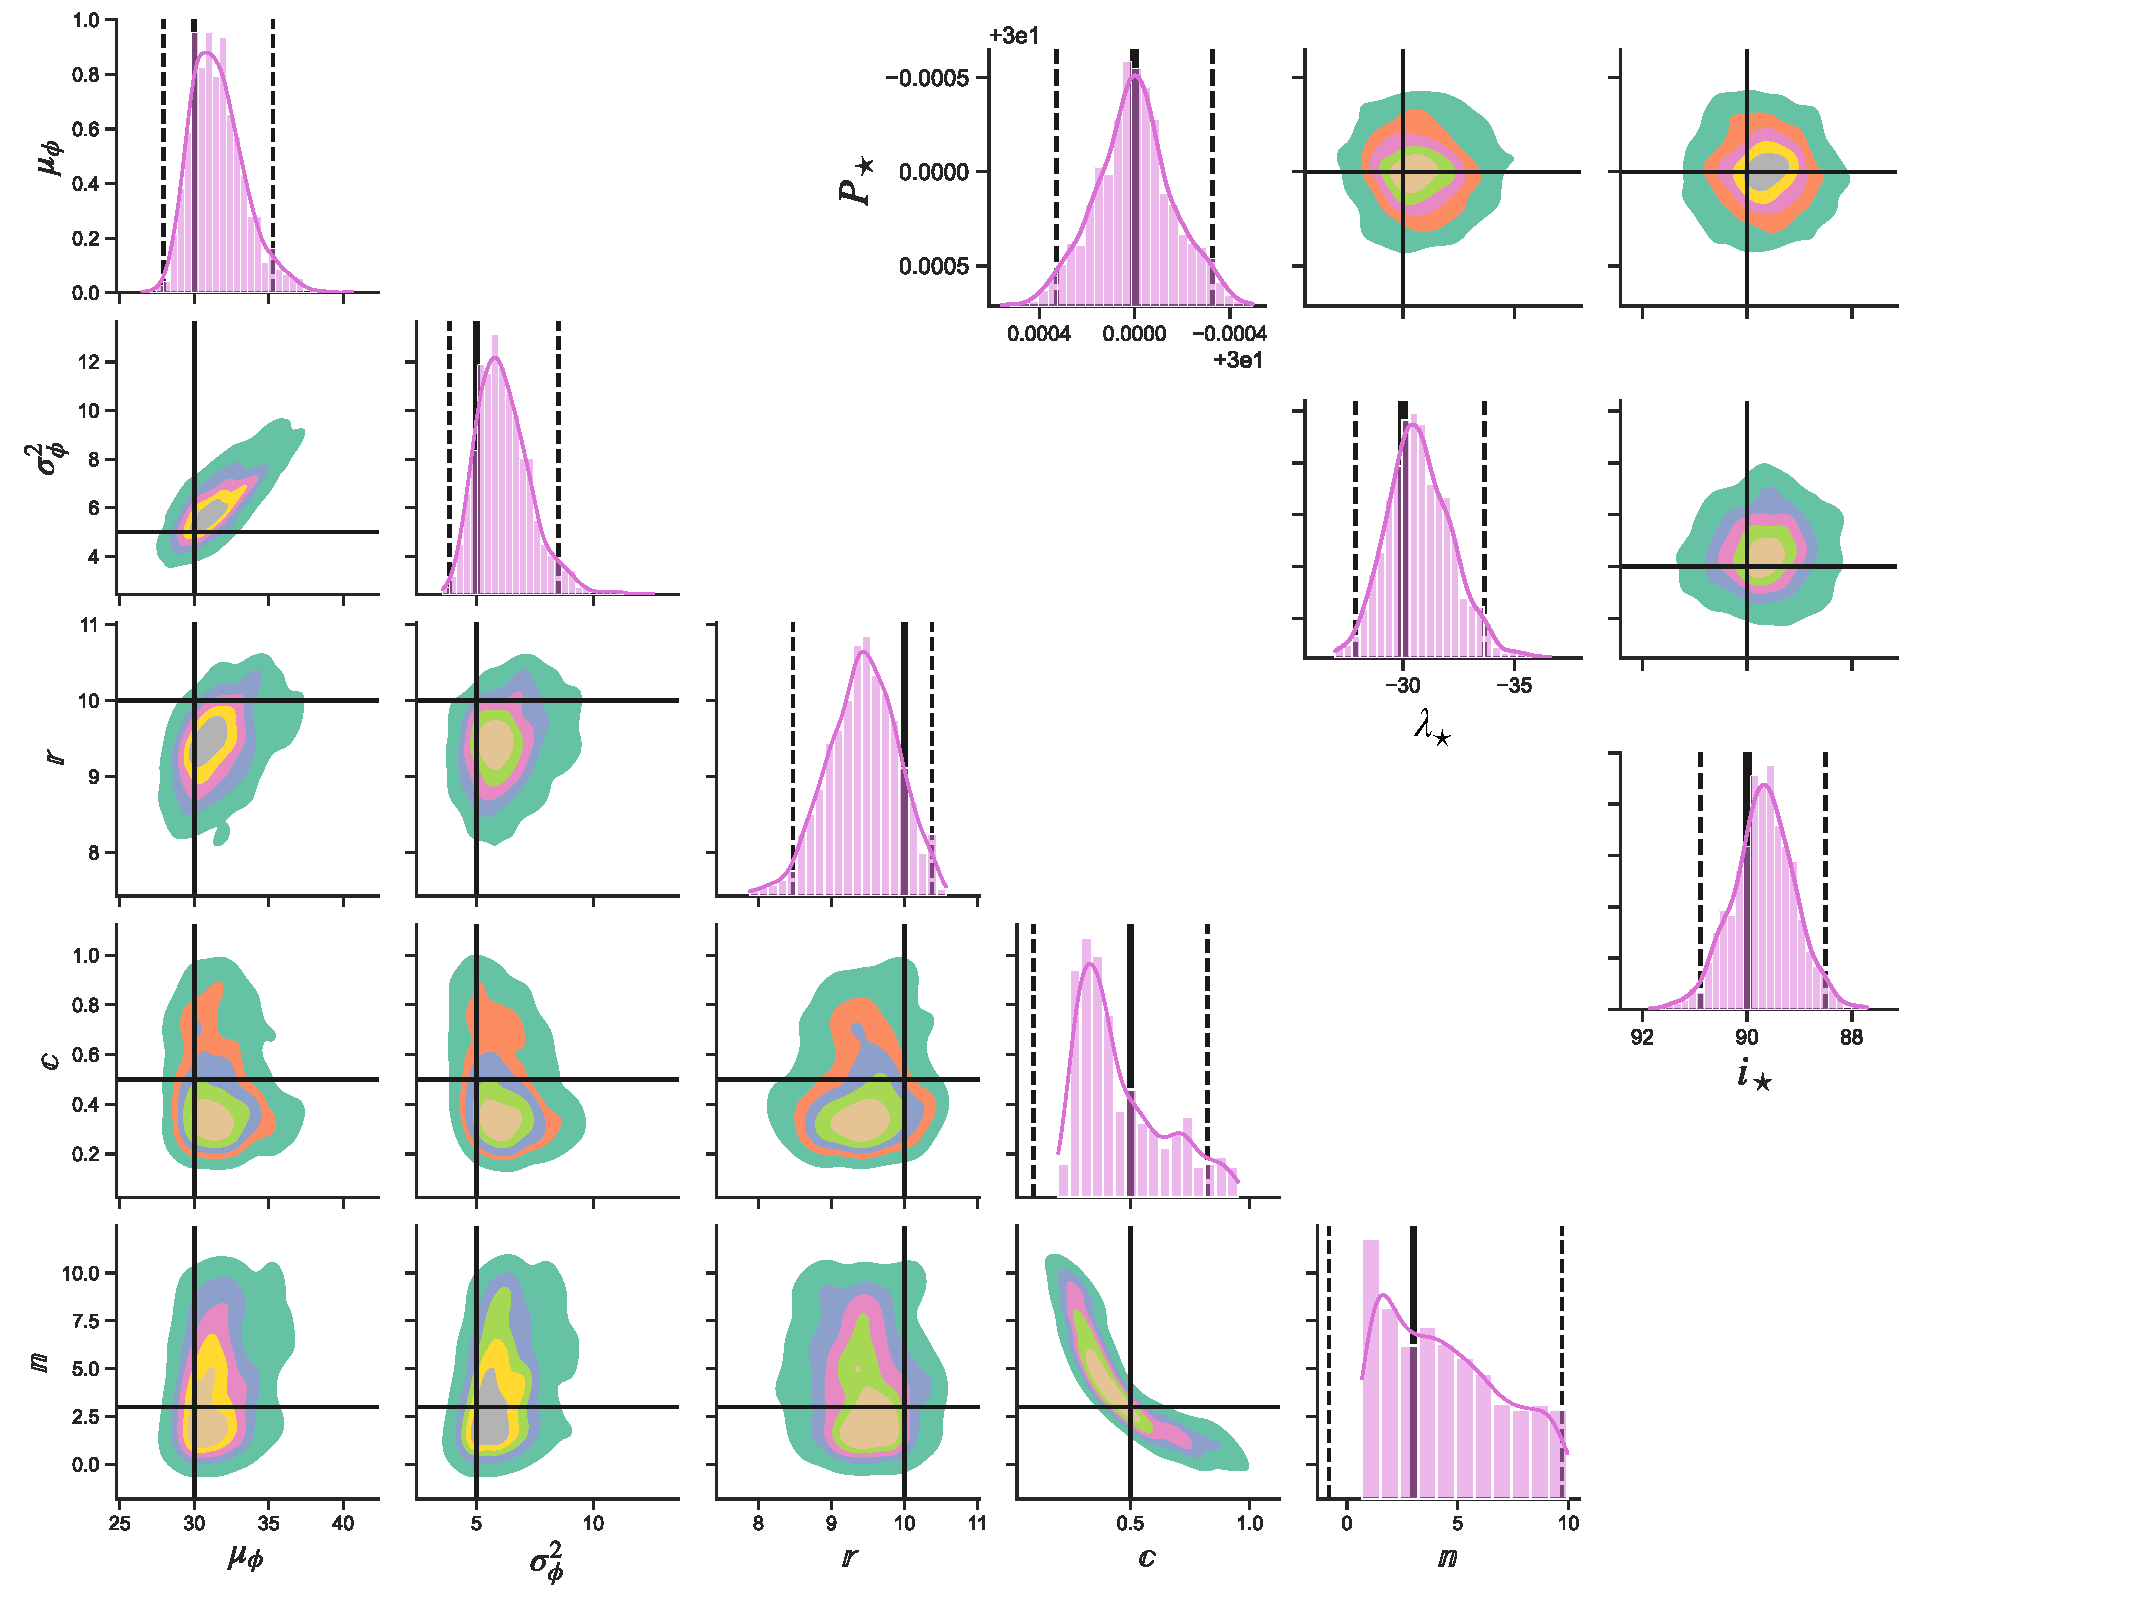
\includegraphics[width=\linewidth]{figures/experiment-1-corner-gp-star.pdf}
        \caption{
            Posterior distributions for the all the parameters $\pmb{\Theta}$ for the synthetic data run 
            (Table \ref{tab:LongPriors} and Figure \ref{fig:experiment-1-map}). The axes span the entire prior volume, and 
            the black lines indicate the true (input) values, the dashed black lines indicate 2 standard deviations.
        }
        \label{fig:experiment-1-map-corner-all}
    \end{centering}
\end{figure*}
%
\begin{figure*}[hbt!]
    % \script{experiment-1-true-map.py}
    \begin{centering}
        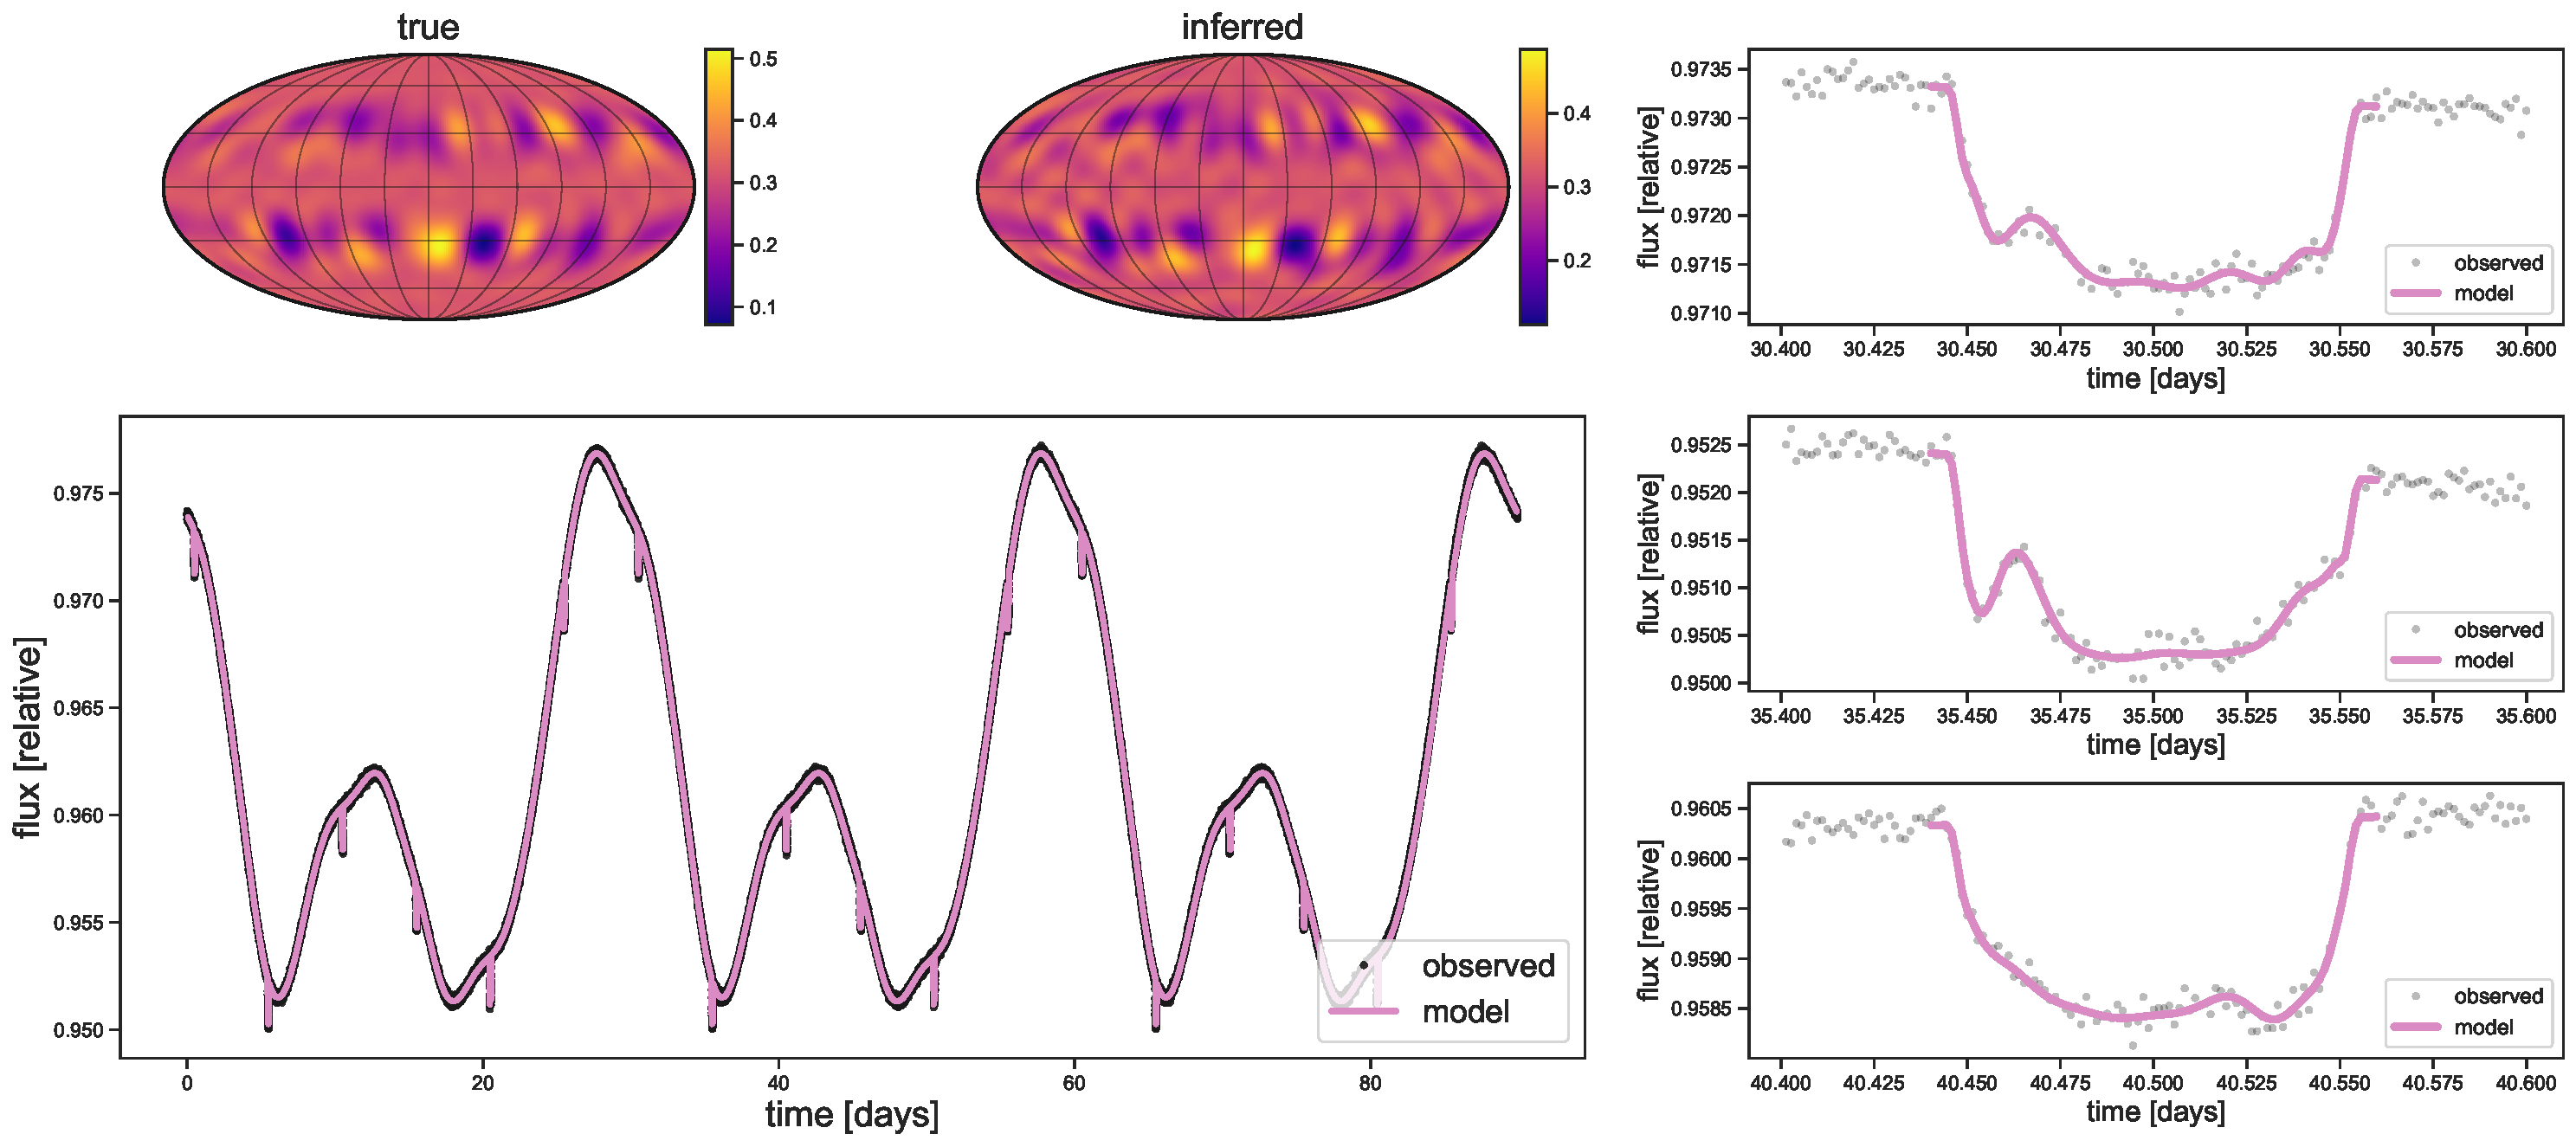
\includegraphics[width=\linewidth]{figures/experiment-1-map-comparison.pdf}
        \caption{
            Comparison of true and inferred stellar surface maps, light curve fit, and transit details. Top panel: the true stellar surface map used to 
            generate synthetic data and the inferred stellar surface map, representing the mean of 1000 posterior samples. Color scales represent spot 
            intensity. The similarity between true and inferred maps demonstrates the model's capability to recover the overall spot distribution. Bottom panel:
            Full light curve comparison. Black points show the synthetic data with added noise. The pink line represents the best-fit model, 
            computed as the mean of 1000 posterior samples. Right panel (three rows): zoom-in views of three consecutive transits. Black points are data, 
            pink lines show the best-fit model. Note the spot-crossing events visible as brief brightness increases during transits. 
            The light curve fit shows strong agreement with the data over the full time series, while the transit close-ups highlight the model's ability 
            to capture subtle spot-crossing events and their evolution over consecutive transits.
        }
        \label{fig:experiment-1-map-comparison}
    \end{centering}
\end{figure*}
%
To evaluate the effectiveness of our model in recovering the underlying spot distribution, we examined the posterior distributions of spot latitudes 
derived from our synthetic data analysis. Figure \ref{fig:experiment-1-acttive-lats} illustrates these results, and the constraints we can place on 
stellar spot distributions. In Figure \ref{fig:experiment-1-acttive-lats}, each pink curve represents a Beta distribution PDF for spot latitude. 
These curves are generated using parameters sampled from the posterior distributions of $\mu_\phi$ and $\sigma_\phi$, which characterize the 
latitude distribution in our model. The collection of pink curves effectively creates a distribution that quantifies our inferred knowledge about 
how spots are distributed across the stellar surface in our dataset. The variability among these pink curves reflects the uncertainty in our inference. 
Regions where the curves are more tightly clustered indicate greater certainty in our estimates, while areas with more spread suggest higher uncertainty. 
This visualization allows us to assess not just a single "best-fit" distribution, but the full range of plausible distributions consistent with our data and model.
The black curve in Figure \ref{fig:experiment-1-acttive-lats} represents the true underlying distribution used to generate the synthetic spot data, 
with parameters as specified in Table \ref{tab:LongPriors}. The general agreement between the ensemble of pink curves and this 
true distribution is encouraging, demonstrating that our model can successfully recover the input spot latitude distribution within the 
uncertainties of the inference process.
%
\begin{figure*}[hbt!]
    % \script{experiment-1-true-map.py}
    \begin{centering}
        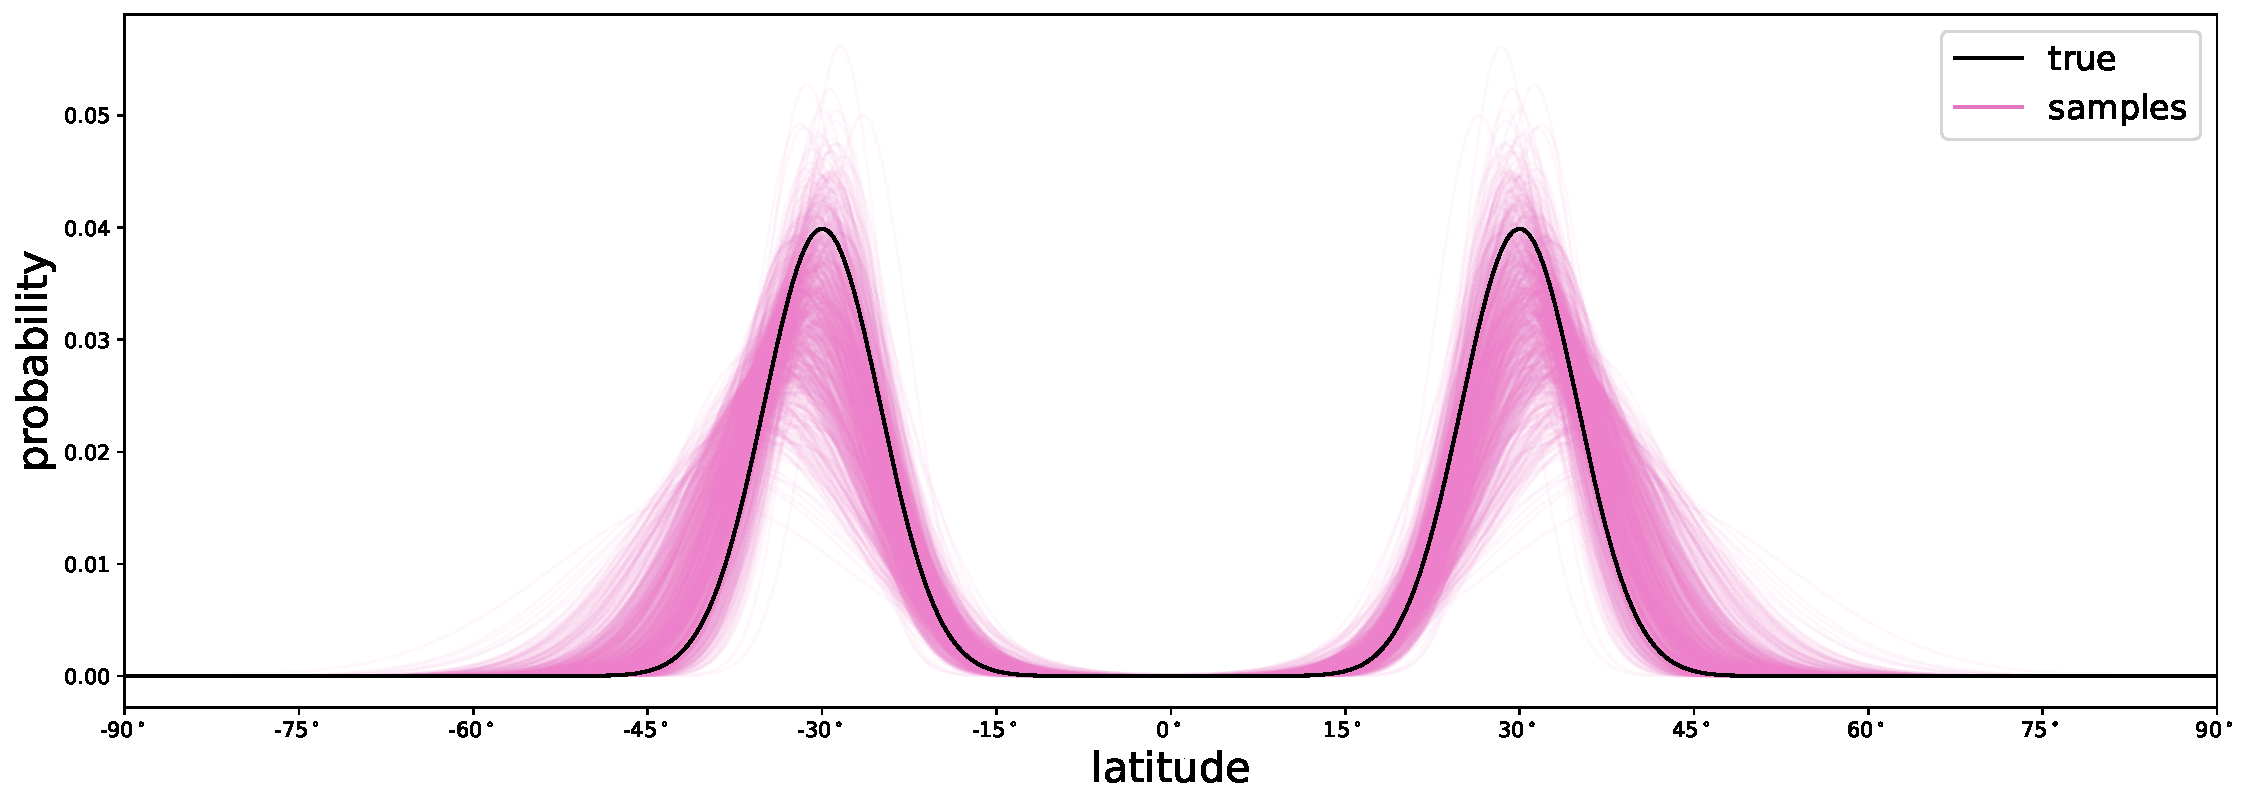
\includegraphics[width=\linewidth]{figures/experiment-1-active-lats.pdf}
        \caption{
            Posterior distributions of spot latitudes derived from synthetic data analysis. The pink curves represent individual Beta distribution 
            probability density functions (PDFs) for spot latitude, each generated using parameters sampled from the posterior distributions of 
            $\mu_\phi$ and $\sigma_\phi$ (Figure \ref{fig:experiment-1-map-corner-all}). The ensemble of pink curves illustrates the range of 
            plausible spot latitude distributions, effectively quantifying our inferred knowledge about spot distribution patterns across the stellar surface 
            in our dataset. The black curve shows the true underlying distribution used to generate the synthetic spot data (parameters given in Table 
            \ref{tab:LongPriors}). Note the general agreement between the inferred distributions and the true distribution, 
            demonstrating the model's ability to recover the input spot latitude distribution within the uncertainties of the inference process.
        }
        \label{fig:experiment-1-acttive-lats}
    \end{centering}
\end{figure*}
%
%
\begin{table}[]
    \vspace{0.5cm}
    \centering
    \caption{The free parameters for the synthetic data in Section \ref{sec:experiment1}, their true values, and their priors.}
    \begin{tabular}{llll}
    \hline
    Parameter                                 & True value            & Prior distribution                   & Inferred value    \\ \hline\hline
    $i_p$                                     & $90^\circ$            & Planetary Inclination                & $90.04^{+0.104}_{-0.089}$                   \\
    $e$                                       & $0.2$                 & $\sim\mathcal{U}(0, 0.5)$            & $0.224 \pm 0.001$                     \\
    $P$                                       & $5$ days              & Period                               & $5.0^{+7\times10^{-6}}_{-6.45\times10^{-6}}$                       \\
    $t_0$                                     & $0.5$                 & $\sim\mathcal{U}(-0.6, 0.6)$         & $0.5^{+10^{-4}}_{-9.8\times10^{-5}}$                       \\
    $R_p / R_\star$                           & $0.04$                & Logarithmic                          & $0.04 \pm 2\times10^{-4}$                         \\ 
    $u_1$                                     & $0.4$                 & $\sim\mathcal{U}(0, 0.6)$            & $0.38^{+0.07}_{-0.06}$                         \\ 
    $u_2$                                     & $0.26$                & $\sim\mathcal{U}(0, 0.4)$            & $0.29 \pm 0.06$                         \\ \hline
    $i_\star$                                 & $90^\circ$            & Stellar Angle                        & $89.68^{+0.6}_{-0.56}$                      \\
    $\lambda_\star$                           & $-30^\circ$           & Stellar Angle                        & $-30.67^{+1.33}_{-1.48}$                           \\
    $P_\star$                                 & $30$ days             & Period                               & $30\pm 2 \times10^{-4}$                       \\ \hline
    $\mathbb{r}$                              & $10^\circ$            & $\sim\mathcal{U}(5, 25)$             & $9.44^{+0.447}_{-0.497}$                           \\
    $\mathbb{c}$                              & $0.5$                 & $\sim\mathcal{U}(0.01, 1)$           & $0.46^{+0.28}_{-0.1}$                               \\
    $\mathbb{n}$                              & $3$                   & $\sim\mathcal{U}(0, 10)$             & $4.45^{+3.53}_{-2.6}$                               \\
    $\mu_\phi$                                & $30^\circ$            & $\sim\mathcal{U}(0, 1)$ on $\mathbb{a}$ and $\mathbb{b}$ & $31.6^{+1.99}_{-1.52}$                               \\
    $\sigma^2_\phi$                           & $5^\circ$             & $\sim\mathcal{U}(0, 1)$ on $\mathbb{a}$ and $\mathbb{b}$ & $6^{+1.2}_{-0.95}$                      \\ \hline
    \label{tab:LongPriors}
    \end{tabular}
\end{table}
%

Finally, it is important to note that all results presented in this analysis have been carefully adjusted to account for the inclination and obliquity 
degeneracy discussed in Section \ref{sec:obl-inc}. As discussed earlier, a system with stellar inclination $i_\star$ and obliquity $-\lambda_\star$ 
produces identical light curves to a system with inclination $180^\circ-i_\star$ and obliquity $\lambda_\star$. In our sampling process, 
when we encounter a solution that gives the obliquity $\lambda_\star$ instead of $-\lambda_\star$, we systematically transform the results. 
Specifically, we change the inclination to $180^\circ-i_\star$ and flip the stellar surface map upside down for visualization purposes. 
This approach ensures consistency in our reported results and allows for meaningful comparisons across different systems or models. 
By explicitly addressing this degeneracy, we provide a more robust and physically interpretable set of results, avoiding potential ambiguities in the 
orientation of the stellar spin axis relative to the planetary orbit.


\section{The Case of TOI-3884}
\label{sec:toi3884}
In this section, we present the results of the model application on TESS light curves of TOI-3884. While TOI-3884 presents a relatively straightforward case, 
it serves as an excellent testbed for demonstrating the capabilities and functionality of our model. By applying our model to TOI-3884, we aim to validate 
its performance on a well-understood system, highlight its ability to extract meaningful information from a real light curve, 
and lay the groundwork for more complex analyses by establishing a baseline of performance.

TOI-3884 (also known as TIC 86263325) was observed by the TESS mission across multiple sectors. The star was monitored for 81 days over a 765-day span, 
using both 30-minute and 2-minute cadences. While Gaia observations show that the TESS aperture for this target isn't significantly contaminated by nearby stars, 
the light curve reveals several transiting spot crossings, indicating stellar activity. Various light curve products were generated for TOI-3884, 
including Simple Aperture Photometry (SAP) 
from the TESS Science Processing Operations Centre and Kepler Spline SAP (KSPSAP) from the Quick-Look Pipeline \citep{Huang2020}. 

TESS revisited TOI-3884 in Sectors 46 and 49, spanning parts of late 2021 and early 2022, using short-cadence observations with 2-minute exposures. 
We used the \texttt{lightkurve} package \citep{lightkurve} to process data from all three sectors, applying strict quality control measures to 
the Pre-search Data Conditioning Simple Aperture Photometry \citep{jenkins2016}.

\begin{figure*}[hbt!]
    % \script{experiment-1-true-map.py}
    \begin{centering}
        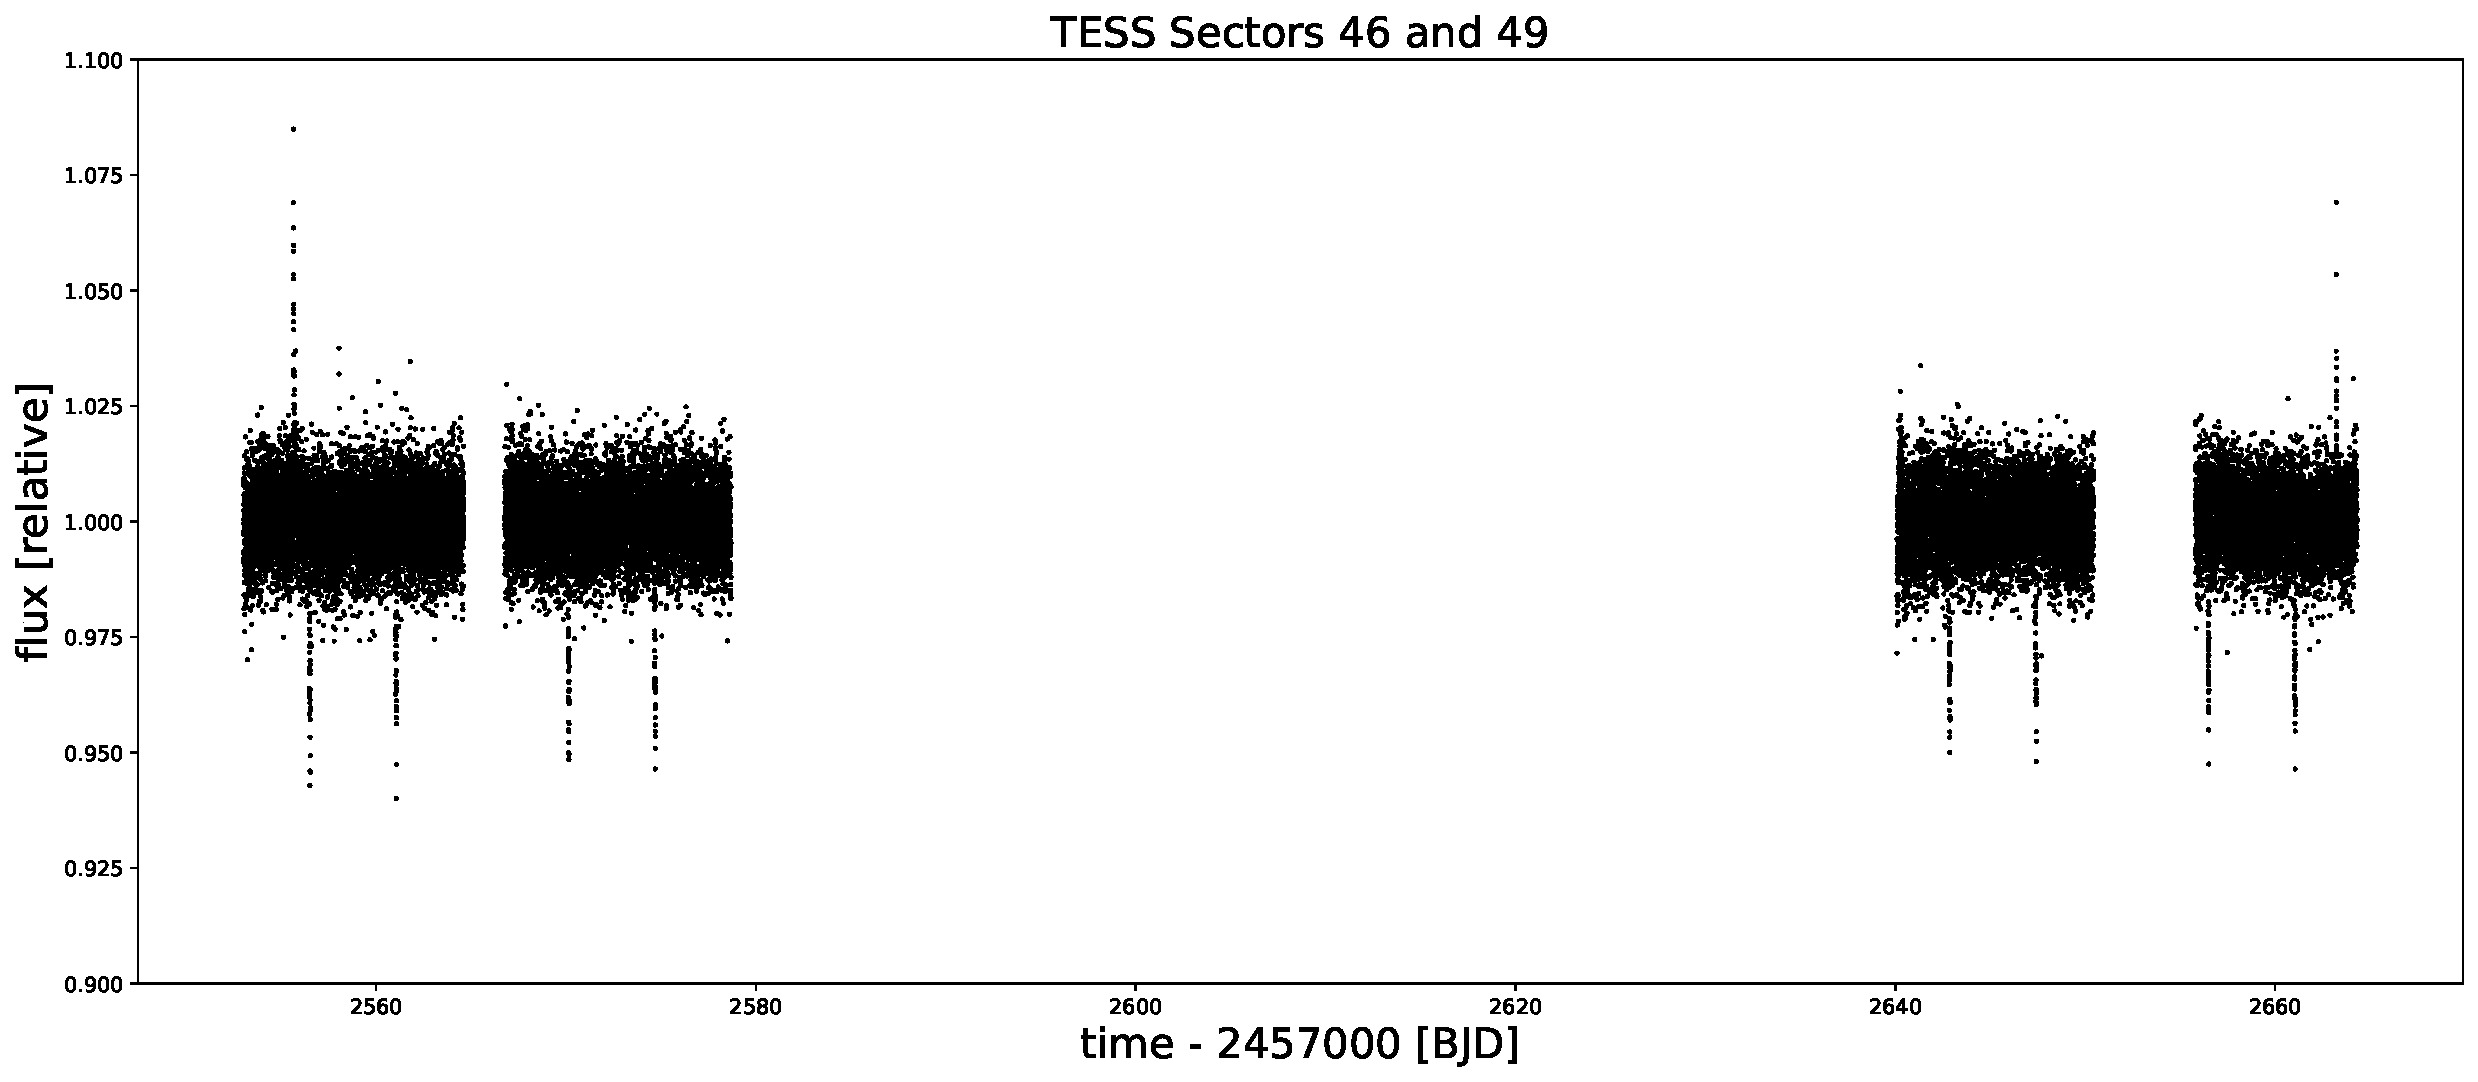
\includegraphics[width=\linewidth]{figures/toi3884-lc.pdf}
        \caption{
            Short 2-minute cadence of the TESS Sectors 46 and 49. 
            Both sets of light curves use the PDCSAP flux.
        }
        \label{fig:toi-3884-pdscap-lc}
    \end{centering}
\end{figure*}

\subsection{Priors for TOI-3884 and TOI-3384 b}

Below, we detail each parameter's prior distribution. We denote the initial values taken from the discovery work of TOI-3884 as 
$\_\rm transit$ taken from \cite{Almenara2022} and the values from the RV observations as $\_\rm RV$ taken from \cite{Libby-Roberts2023}.

The impact parameter $b$ follows a uniform distribution between $-b_{\text{max}}$ and $b_{\text{max}}$, 
where $b_{\text{max}} = R_{\star}/a$ represents the ratio of the stellar radius to the semi-major axis. 
This prior encompasses all possible transit geometries, including grazing transits: $b \sim \mathcal{U}(-b_{\text{max}}, 
b_{\text{max}})$.

The orbital eccentricity $e$ is constrained to physically meaningful values with a uniform prior between 0 (circular orbit) and 1 (parabolic orbit): 
$e \sim \mathcal{U}(0, 1)$.

For the orbital period $P_{\text{orb}}$, we use a tight uniform prior on a scaling factor $f_{P_{\text{orb}}}$ around the known value: 
$f_{P_{\text{orb}}} \sim \mathcal{U}(0.99, 1.01)$, with the actual period derived as $P_{\text{orb}} = P_{\text{orb,transit}} \cdot f_{P_{\text{orb}}}$. 
This allows for small adjustments to the period while maintaining consistency with observed transits.

Similarly, the mid-transit time $t_0$ is parameterized through a scaling factor $f_{t_0} \sim \mathcal{U}(0.9, 1.1)$, 
with the actual time calculated as $t_0 = t_{0,\text{transit}} + P_{\text{orb,transit}} \cdot (f_{t_0} - 1)$. 
This formulation permits the mid-transit time to vary within approximately $\pm10\%$ of the orbital period from the initial estimate.

The planet radius is parameterized in log space with a uniform prior that allows it to vary between half and twice the 
initially estimated value: $\ln(R_p) \sim \mathcal{U}(\ln(R_{p,\text{transit}}/2), \ln(2 \cdot R_{p,\text{transit}}))$.

The orientation of the orbital angular momentum is parameterized through $w_x$ and $w_y$, which follow standard normal 
distributions: $w_x, w_y \sim \mathcal{N}(0, 1)$. 
This provides a uniform distribution over the unit sphere when properly transformed to three dimensions.

The stellar position parameters $\tilde{x}_{\star}$, $\tilde{y}_{\star}$, and $\tilde{z}_{\star}$ similarly follow standard normal 
distributions: $\tilde{x}_{\star}$, $\tilde{y}_{\star},\tilde{z}_{\star} \sim \mathcal{N}(0, 1)$, allowing for uncertainty in the precise position 
of the star.

The limb darkening coefficients for a quadratic limb darkening law are given uniform priors: 
$u_1 \sim \mathcal{U}(0, 0.5)$ and $u_2 \sim \mathcal{U}(0, 0.2)$. These ranges are consistent with typical values 
for main-sequence stars.

The stellar rotation period $P_{\text{rot}}$ is parameterized as a multiple of the estimated 
value: $f_{P_{\text{rot}}} \sim \mathcal{U}(0.2, 1.8)$ with $P_{\text{rot}} = f_{P_{\text{rot}}} 
\cdot 10$, allowing the rotation period to vary between 20\% and 180\% of the initial estimate. This translates to the uniform 
distribution from 2 to 18 days.

The stellar mass follows a log-normal distribution derived from density measurements: 
$\ln(M_{\star}) \sim \mathcal{N}(\ln(\rho_{\rm RV} / \rho_{\odot}), \sigma_{\rho_{\rm RV}} / \rho_{\rm RV})$. 
This prior incorporates observational constraints on the stellar density while properly accounting for the uncertainty.
The radius of the star stays fixed at 1 $R_\odot$.

For the Gaussian Process (GP) kernel parameters modeling stellar activity, we employ uniform priors: the radius of spots 
$\mathbb{r} \sim \mathcal{U}(10.0, 60.0)$, the contrast $\mathbb{c} \sim \mathcal{U}(0.01, 0.9)$, 
the number of spots $\mathbb{n} \sim \mathcal{U}(0.1, 10.0)$, the mean of the latitude distribution $\mu_\phi \sim \mathcal{U}(0.1, 80.0)$, 
and the variance of the latitude distribution $\sigma^2_\phi \sim \mathcal{U}(0.1, 20.0)$.

All parameters constrained to specific ranges are implemented using logit/inverse-logit transformations with appropriate 
Jacobian adjustments in the log-probability calculations to maintain proper probability distributions.

\subsection{Addressing Multimodality with Parallel Tempering}

The posterior distribution of our model exhibits significant multimodality, presenting substantial challenges for 
conventional sampling methods. This multimodality arises from several sources inherent to transit modeling. 
First, the degeneracy between impact parameter and planet radius creates multiple regions of high posterior probability. 
Second, the periodic nature of orbital elements introduces symmetries in the likelihood landscape, particularly when stellar 
activity signals interact with planetary transit signatures. Third, the parameterization of stellar rotation and activity through 
our model introduces additional complexity with multiple viable configurations that can explain the observed data equally well.

Standard Markov Chain Monte Carlo (MCMC) methods such as Ensemble Sampling (e.g., \texttt{emcee} \cite{emcee}) or Hamiltonian Monte Carlo (HMC; \cite{Hoffman2011}) struggle 
in this multimodal landscape. Ensemble samplers can become trapped in local modes, failing to explore the full posterior 
distribution even with large numbers of walkers. This "mode-trapping" problem is particularly severe in our high-dimensional 
parameter space, where narrow connecting pathways between modes create bottlenecks for efficient sampling. Similarly, 
HMC methods, while excellent for exploring complicated geometries within a single mode, typically fail to transition between 
widely separated modes due to the momentum-based dynamics that govern their exploration.

To overcome these limitations, we utilized Parallel Tempering (PT), also known as replica exchange MCMC. 
This method simultaneously runs multiple MCMC chains at different "temperatures," where temperature controls the 
degree to which the posterior is flattened. At high temperatures, the likelihood is down-weighted, allowing chains to 
move more freely across the parameter space and easily traverse valleys between modes. At the lowest temperature 
($T=1$), the chain samples from the true posterior of interest.

The key innovation in PT is the periodic exchange of states between chains at adjacent temperatures. 
These exchanges allow configurations discovered at high temperatures to propagate down to the cold chain, 
effectively enabling jumps between modes that would be extremely rare in standard MCMC. We used the implementation
of PT in \texttt{ptemcee} \citep{ptemcee}. \texttt{ptemcee} handles these exchanges using the Metropolis criterion:

\begin{equation}
    \label{eq:ptemcee}
    P_{\rm exchange} = \min\left(1, \exp\left[\left(\frac{1}{T_i} - \frac{1}{T_j}\right)\right.\right.\\
    \left.\left.\left(\ln p(\theta_j|\mathcal{D}) - \ln p(\theta_i|\mathcal{D})\right)\right]\right)
\end{equation}

where $T_i$ and $T_j$ are the temperatures of adjacent chains, and $\theta_i$ and $\theta_j$ are their respective states.
Our implementation used a ladder of 8 temperatures geometrically spaced between $T=1$ and $T=\infty$, with exchange attempts proposed 
every 10 iterations. To validate adequate sampling across modes, we monitored the exchange acceptance rates between adjacent 
temperature levels, aiming for rates between 10\% and 40\%.

\subsection{Results}
The full posterior distributions for all model parameters are summarized in Table \ref{tab:ResultsT0i3884}. Here, we highlight the 
most significant results.

The spot model strongly favors a high-latitude feature with an angular radius of $\mathbb{r} = 26.77^{+9.7}_{-8.7}$ degrees, 
covering approximately 2.5-10\% of the stellar surface. 

Figure \ref{fig:spot_parameters} presents the posterior distributions and correlations of the key parameters in our spot model. 
Our analysis strongly favors a high-latitude spot configuration with the spot center located at $\mu_{\phi} = {75.3}^{+3.7}_{-4.2}$ 
degrees, indicating a near-polar feature. The spot contrast parameter $\mathbb{c} = 0.049^{+0.028}_{-0.013}$ corresponds to a 
moderate temperature difference between the spot and surrounding photosphere, consistent with typical values observed on active M 
dwarfs. The angular variance in longitude $\sigma^2_{\phi}$ shows bimodality, with peaks at approximately $5^{\circ}$ 
and $15^{\circ}$, indicating two distinct possible spot configurations with different latitudinal spreads. 
The close correlation between stellar inclination and spot latitude reflects the geometric constraints imposed by the transit 
observations. Collectively, these parameters paint a picture of TOI-3884 as an active star with significant polar spotting.

\begin{figure*}[hbt!]
    \centering
    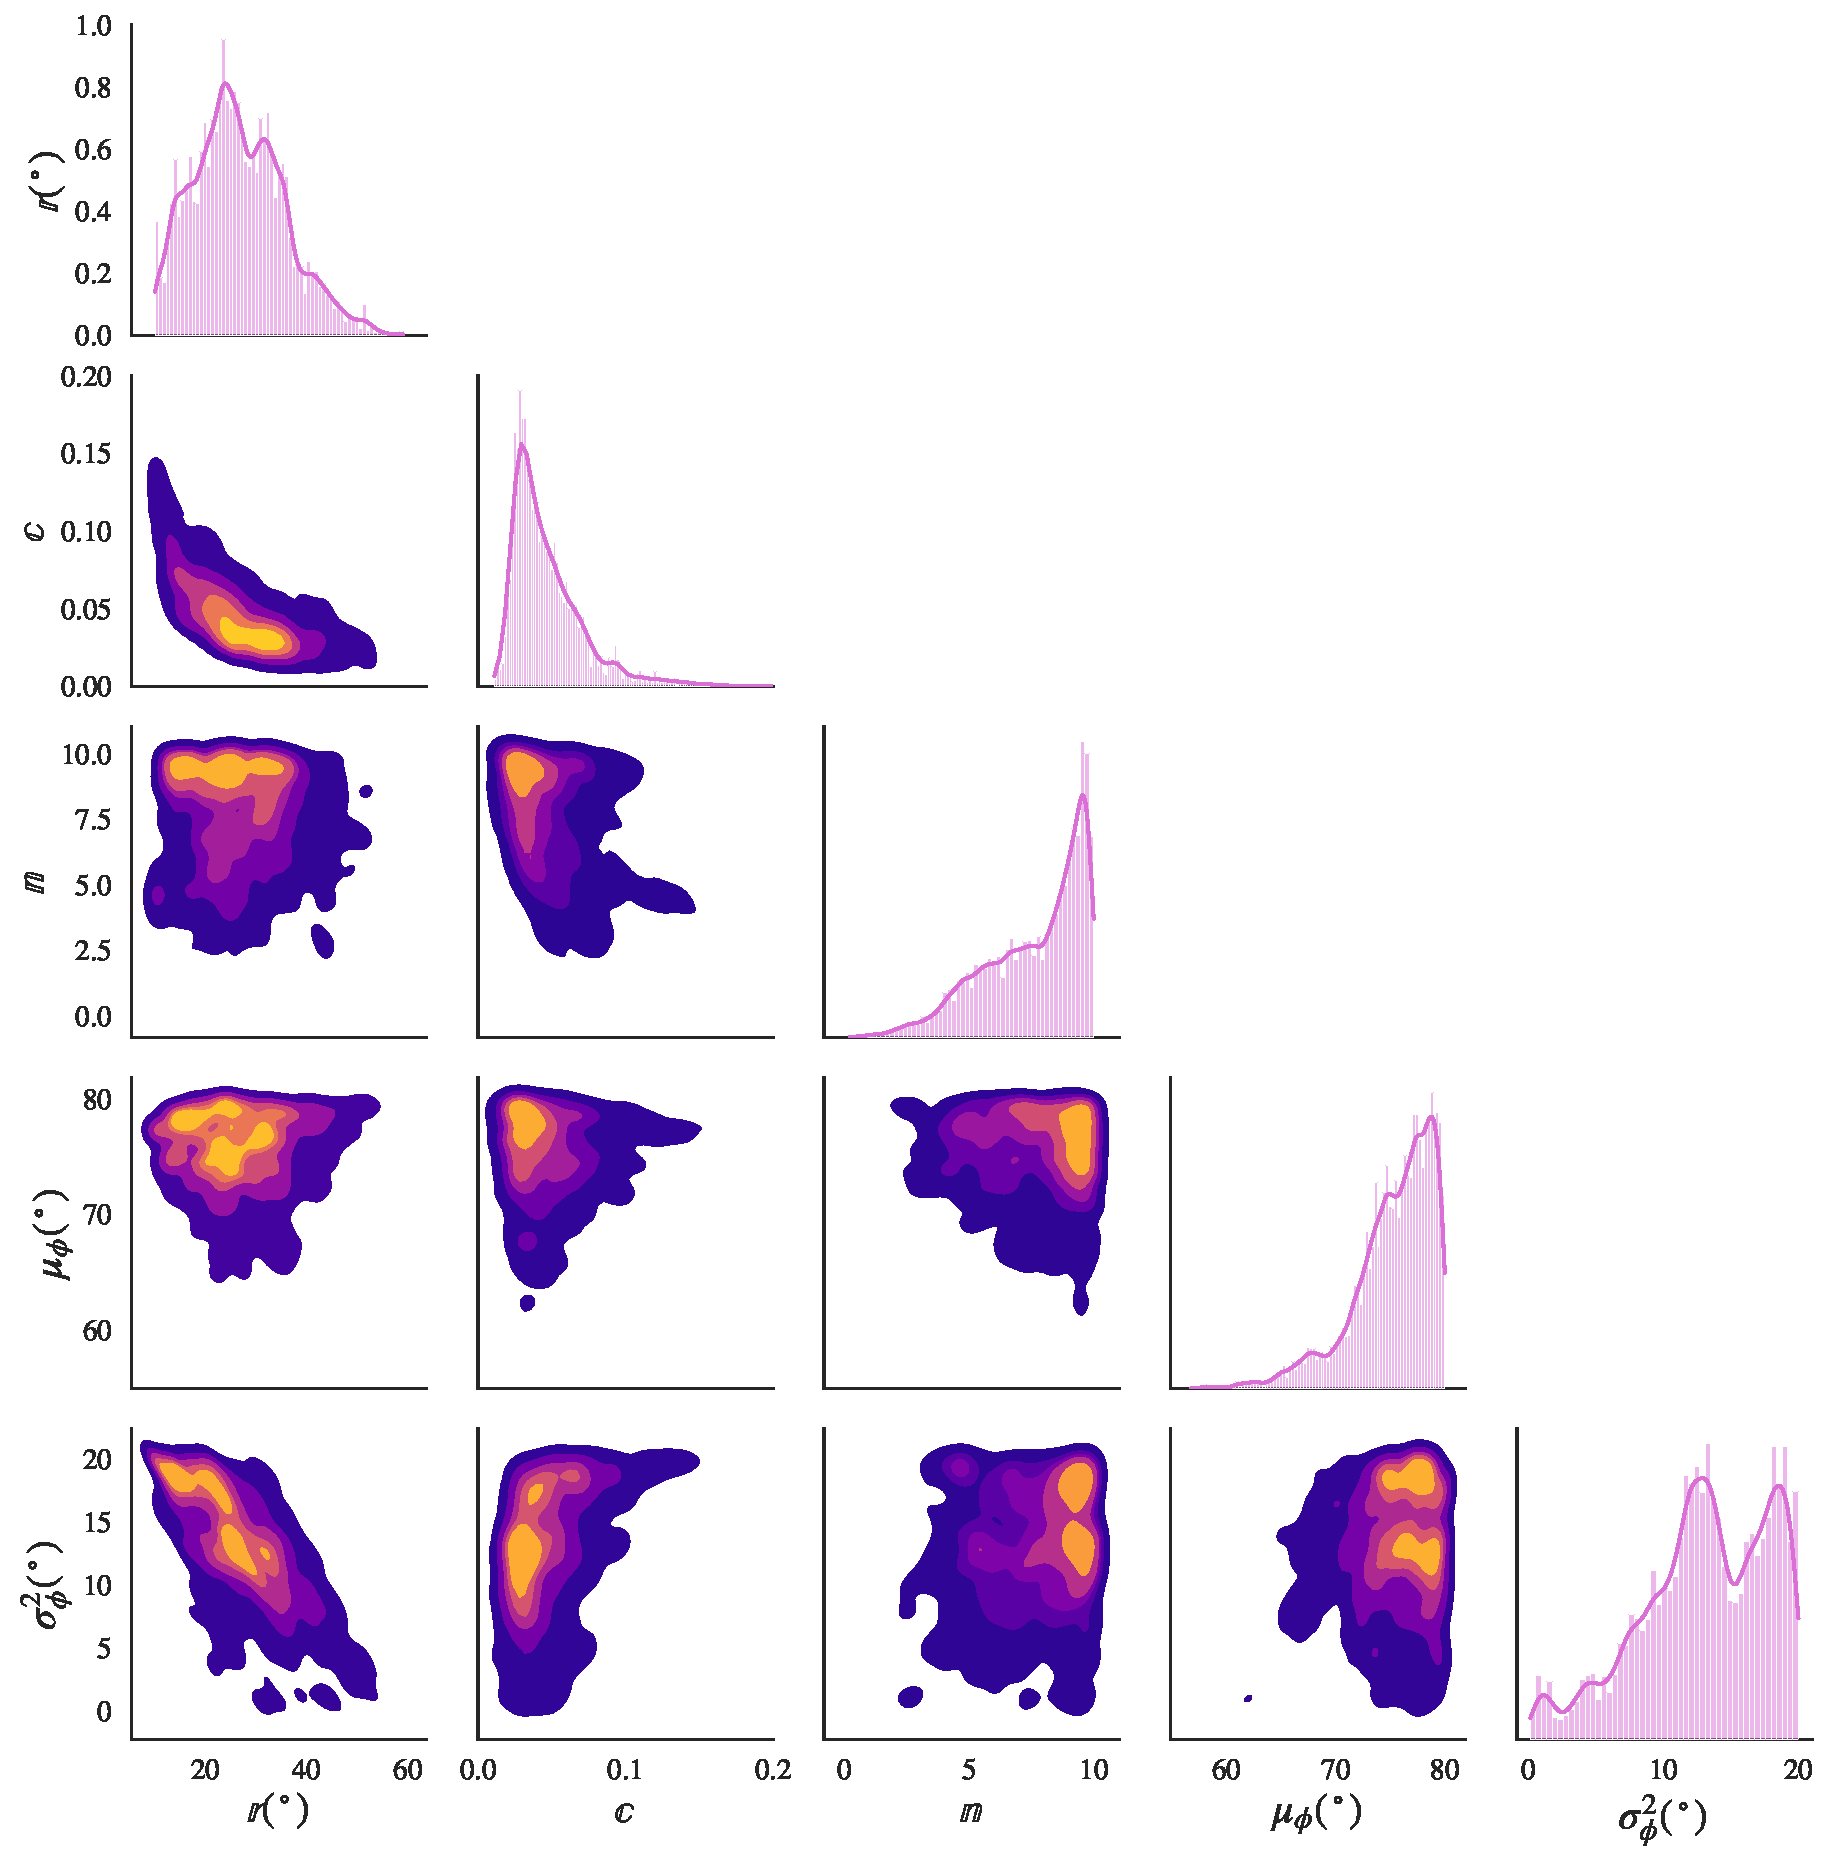
\includegraphics[width=\textwidth]{figures/toi3884-corner-gps.pdf}
    \caption{Corner plot showing the posterior distributions and correlations for the spot model parameters. 
    The diagonal panels display the marginalized posterior distributions for each parameter: the spot size 
    $\mathcal{r}$ ($^{\circ}$), spot contrast $\mathcal{c}$, number of spots $\mathcal{n}$, spot latitude $\mu_{\phi}$ ($^{\circ}$), 
    and the angular variance in latitude $\sigma^2_{\phi}$ ($^{\circ}$). The spot latitude is concentrated at high values around 
    $75^{\circ}$--$80^{\circ}$, 
    confirming the presence of a near-polar spot. The spot contrast is relatively modest with most of the probability mass below
     0.1. The number of spots tends toward values between 7.5 and 10, suggesting a relatively small number of spots.}
    \label{fig:spot_parameters}
\end{figure*}

Our analysis of the spot latitude distribution is illustrated in Figure \ref{fig:spot_latitude}. This figure shows the posterior 
probability distribution of spot latitudes derived from our MCMC analysis. The black line represents the mean distribution, 
while the individual pink lines show a subset of 1000 posterior samples, highlighting the inherent variability in our constraints. 
The distribution exhibits two prominent peaks centered at approximately $-75^{\circ}$ and $+75^{\circ}$ latitude, 
with negligible probability near the equator.

While we cannot definitively determine whether the spot is in the northern or southern hemisphere based on the transit data alone, 
the presence of either configuration would lead to similar physical interpretations regarding the underlying stellar dynamo processes. 
This latitude distribution, combined with the other spot parameters discussed previously, presents compelling evidence for strong, 
organized magnetic fields concentrated at the rotational poles of TOI-3884.

\begin{figure*}[hbt!]
    \centering
    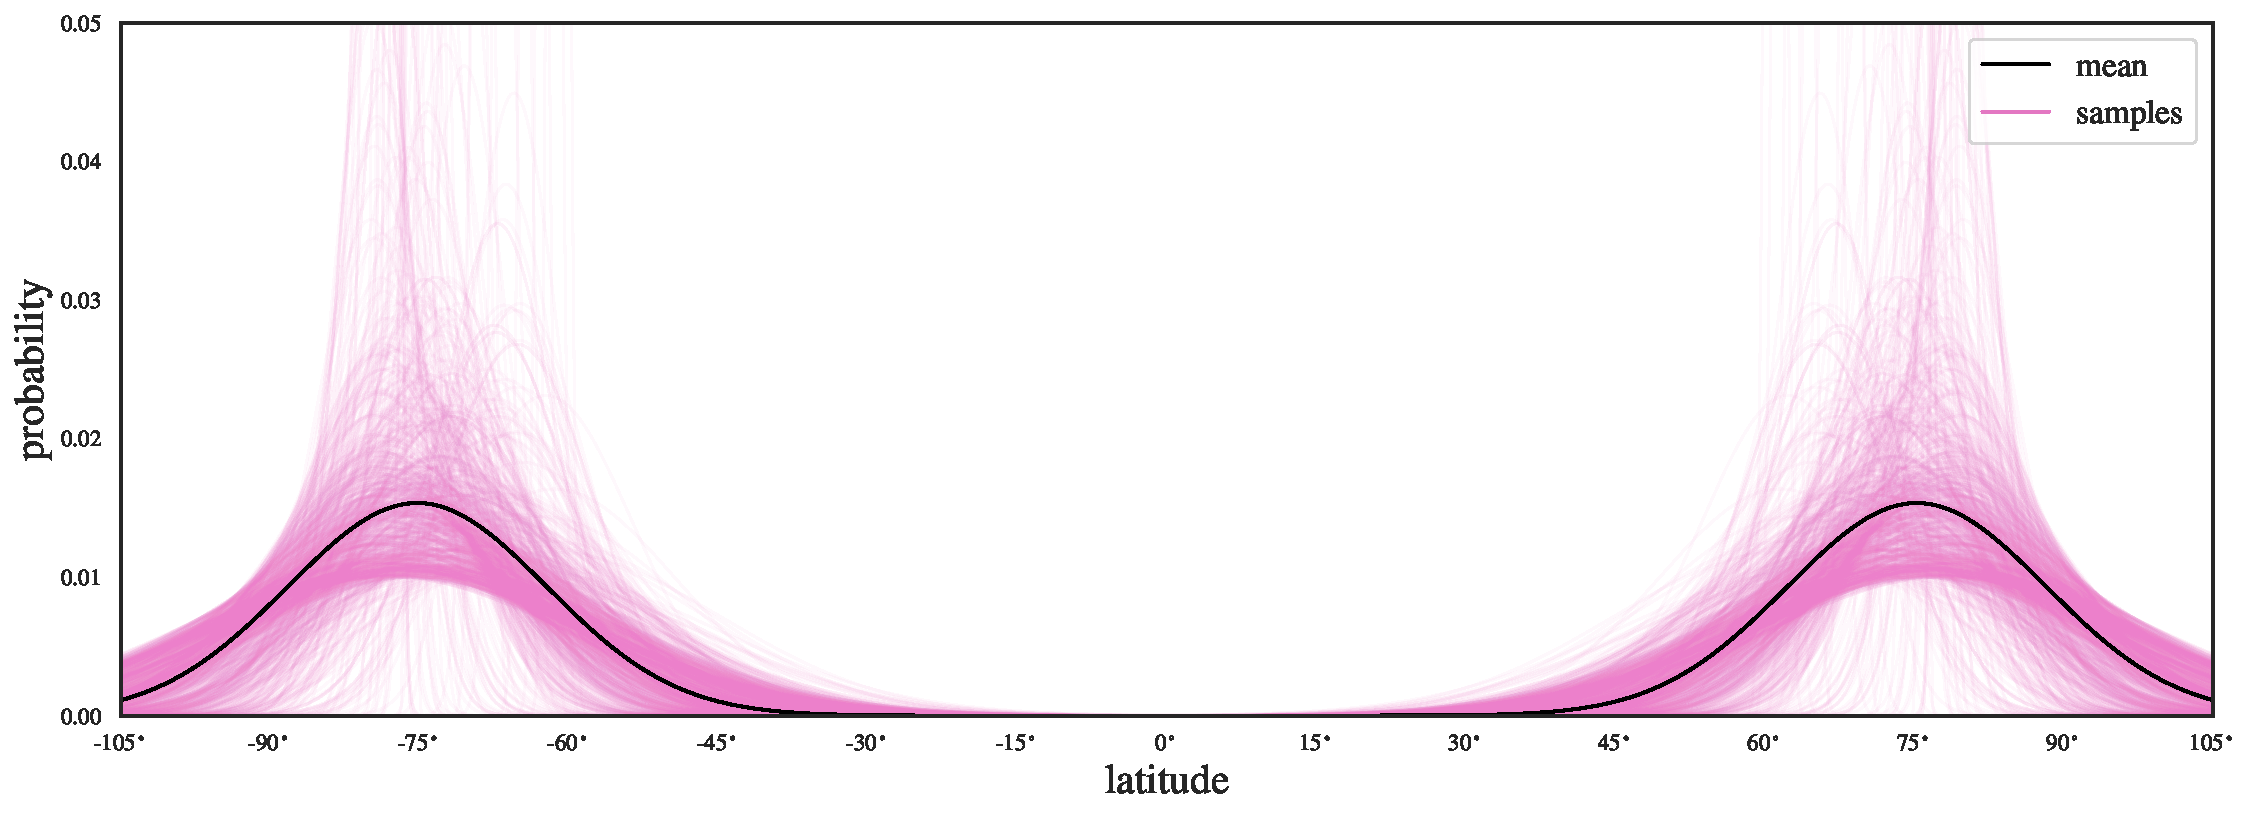
\includegraphics[width=\textwidth]{figures/toi3884-active-lats.pdf}
    \caption{Posterior probability distribution of spot latitudes for TOI-3884. The black line shows the mean distribution, 
    while the pink lines represent individual posterior samples from our MCMC analysis. The distribution peaks at high latitudes 
    ($\pm75^{\circ}$) with minimal probability near the equator, indicating a strong preference for near-polar spots.
    The symmetry across 
    the equator reflects the inherent degeneracy in determining the hemisphere of spot locations from transit data alone.}
    \label{fig:spot_latitudes}
\end{figure*}

The stellar inclination angle was found to be $i_\star = {34.8}^{+5.62}{-6.17}$ degrees, indicating that the stellar rotation 
axis is considerably inclined from the line of sight. More notably, the sky-projected spin-orbit angle (stellar obliquity) was 
determined to be $\lambda\star = {80.37}^{+49.6}_{-27.5}$ degrees.
The stellar rotation period was constrained to $P_\text{rot} = 9.07^{+0.45}_{-0.51}$ days, which places TOI-3884 among the 
more rapidly rotating M dwarfs, consistent with its observed activity level and estimated age.

We find a planetary radius of $R_p = 0.188 \pm 3\times10^{-3}$ $R_\earth$ and an orbital period of 
$P_\text{orb} = 4.5446^{+2.7\times10^{-5}}_{-2.4\times10^{-5}}$ days. 

\begin{table}[]
    \vspace{0.5cm}
    \centering
    \caption{The free parameters for TOI-3884 data in Section \ref{sec:toi3884}, their true values, and their priors.}
    \begin{tabular}{llll}
    \hline
    Parameter                                 & Inferred value    \\ \hline\hline
    $i_p (^\circ)$                                     & $90.17^{+0.52}_{-0.78}$                   \\
    $e$                                       & $0.14^{+0.19}_{-0.07}$                     \\
    $P (\rm days)$                                       & $4.5446^{+2.7\times10^{-5}}_{-2.4\times10^{-5}}$                       \\
    $t_0 (\rm days)$                                     & $2556.51\pm 4\times 10^{-4}$                       \\
    $R_p / R_\star$                           & $0.188 \pm 3\times10^{-3}$                         \\ 
    $u_1$                                     & $0.14^{+0.15}_{-0.07}$                         \\ 
    $u_2$                                     & $0.09 \pm 0.06$                         \\ 
    $v\sin i (\rm kms^{-1})$                                & $1.69^{+0.11}_{-0.09}$                       \\ \hline
    $i_\star (^\circ)$                                 & $34.8^{+5.62}_{-6.17}$                      \\
    $\lambda_\star (^\circ)$                           & $80.37^{+49.6}_{-27.5}$                           \\
    $P_\star (\rm days)$                                 & $9.07^{+0.45}_{-0.51}$                       \\ 
    $\rho_\star (\rm gcm^{-3})$                              & $15.18^{+1.98}_{-1.75}$                      \\ \hline
    $\mathbb{r} (^\circ)$                              & $26.77^{+9.7}_{-8.7}$                           \\
    $\mathbb{c}$                              & $0.049^{+0.028}_{-0.013}$                               \\
    $\mathbb{n}$                              & $7.58^{+1.39}_{-2.85}$                               \\
    $\mu_\phi (^\circ)$                                & $75.24^{+2.67}_{-4.11}$                               \\
    $\sigma^2_\phi (^\circ)$                           & $12.99^{+4.91}_{-5.08}$                      \\ \hline
    \label{tab:ResultsT0i3884}
    \end{tabular}
\end{table}
%

\bibliography{bib}

\end{document}
